%%%% Proceedings format for most of ACM conferences (with the exceptions listed below) and all ICPS volumes.
\documentclass[format=sigconf,10pt]{acmart}
%%%% As of March 2017, [siggraph] is no longer used. Please use sigconf (above) for SIGGRAPH conferences.

%%%% Proceedings format for SIGPLAN conferences 
% \documentclass[sigplan, anonymous, review]{acmart}

%%%% Proceedings format for SIGCHI conferences
% \documentclass[sigchi, review]{acmart}

%%%% To use the SIGCHI extended abstract template, please visit
% https://www.overleaf.com/read/zzzfqvkmrfzn


\usepackage{booktabs} % For formal tables
\usepackage{algorithm} % For pseudo code
\usepackage[noend]{algpseudocode} % For pseudo code
\usepackage{geometry}
\usepackage[colorinlistoftodos]{todonotes}

\usepackage{subcaption} % For skip list figs

\pagenumbering{arabic}

% Copyright
%\setcopyright{none}
%\setcopyright{acmcopyright}
%\setcopyright{acmlicensed}
\setcopyright{rightsretained}
%\setcopyright{usgov}
%\setcopyright{usgovmixed}
%\setcopyright{cagov}
%\setcopyright{cagovmixed}

%%%%% Begin - For Camera Ready %%%%
% % DOI
% \acmDOI{10.475/123_4}

% % ISBN
% \acmISBN{123-4567-24-567/08/06}

% %Conference
% \acmConference[ANCS'18]{ACM/IEEE Symposium on Architectures for Networking and Communications Systems}{May 2018}{Ithaca, NY, USA}
% \acmYear{2018}
% \copyrightyear{2018}

% \acmArticle{4}
% \acmPrice{15.00}
%%%%% End - For Camera Ready %%%%

% These commands are optional
%\acmBooktitle{Transactions of the ACM Woodstock conference}
% \editor{Jennifer B. Sartor}
% \editor{Theo D'Hondt}
% \editor{Wolfgang De Meuter}


\begin{document}
\title{Scalable and Programmable Packet Scheduling}
\subtitle{Paper \#N, 12 pages}


% \author{Anthony Dalleggio}
% %\authornote{Anthony's note}
% \orcid{1234-5678-9012}
% \affiliation{%
%   \institution{New York University}
%   \city{New York}
%   \state{N.Y.}
% }
% \email{ad3002@nyu.edu}

% \author{Stephen Ibanez}
% %\authornote{Stephen's Note}
% \affiliation{%
%   \institution{Stanford University}
%   \city{Stanford}
%   \state{C.A.}
% }
% \email{sibanez@stanford.edu}

% \author{Gordon Brebner}
% \affiliation{%
%   \institution{Xilinx Labs}
%   \city{San Jose}
%   \state{C.A.}
% }
% \email{gjb@xilinx.com}

% \author{Nick McKeown}
% \affiliation{%
%   \institution{Stanford University}
%   \city{Stanford}
%   \state{C.A.}
% }
% \email{nickm@stanford.edu}

% \author{Jonathan Chao}
% \affiliation{%
%   \institution{New York University}
%   \city{New York}
%   \state{N.Y.}
% }
% \email{chao@nyu.edu}

% \author{Yang Xu}
% \affiliation{%
%   \institution{New York University}
%   \city{New York}
%   \state{N.Y.}
% }
% \email{yang@nyu.edu}

% The default list of authors is too long for headers.
%\renewcommand{\shortauthors}{A. Dalleggio et al.}


\begin{abstract}
Today's programmable switches allow software developers to define how headers are processed; but so far, they do not allow us to define new packet scheduling algorithms. The PIFO (Push-In-First-Out) queue was recently proposed as a convenient (and practical) abstraction to represent many different scheduling algorithms. PIFOs differ from traditional scheduling mechanisms because they decide the packet's scheduling order at the time of enqueue (when the packet arrives) rather than when the packet departs. This paper proposes a design for the first practical programmable traffic manager using the PIFO as a scheduling primitive. We describe and evaluate a novel PIFO implementation designed for FPGA targets that can scale to support 10Gb/s line rate ports or higher. We prototype our programmable traffic manager on the NetFPGA SUME platform and demonstrate that it can be used to implement various common scheduling algorithms. Our PIFO implementation is available as an open-source project to reproduce and extend our results.
\end{abstract}

%
% The code below should be generated by the tool at
% http://dl.acm.org/ccs.cfm
% Please copy and paste the code instead of the example below.
%
% \begin{CCSXML}
% <ccs2012>
% <concept>
% <concept_id>10003033.10003068.10003069.10003072</concept_id>
% <concept_desc>Networks~Packet scheduling</concept_desc>
% <concept_significance>500</concept_significance>
% </concept>
% <concept>
% <concept_id>10003033.10003099.10003102</concept_id>
% <concept_desc>Networks~Programmable networks</concept_desc>
% <concept_significance>500</concept_significance>
% </concept>
% <concept>
% <concept_id>10003033.10003034.10003038</concept_id>
% <concept_desc>Networks~Programming interfaces</concept_desc>
% <concept_significance>300</concept_significance>
% </concept>
% </ccs2012>
% \end{CCSXML}

% \ccsdesc[500]{Networks~Packet scheduling}
% \ccsdesc[500]{Networks~Programmable networks}
% \ccsdesc[300]{Networks~Programming interfaces}

% \keywords{Programmable Networks, Packet Scheduling, FPGA}

\settopmatter{printfolios=true}
\maketitle

\section{Introduction}

%\todo[inline]{\\
% What is programmable scheduling? \\
%% Why we need programmable scheduling? \\
% Why isn't scheduling already programmable? \\
% Why FPGAs? \\
%}

There is much talk about using the P4 language~\cite{p4:2014} to define how packets are processed by a programmable switch~\cite{p4org, p4runtime, Stratum}. P4 is being used by networking researchers and the networking industry to define the forwarding pipeline of software switches~\cite{Pisces}, FPGAs~\cite{SDNet}, programmable ASICs~\cite{Tofino, Xpliant} and NICs~\cite{Netronome}. To date, though, the P4 language has been limited to defining how packets are parsed, and the `match + action' pipeline. Much less attention has been focused on traffic management and how individual packets are scheduled. For example, programmable ASICs allow a packet scheduling algorithm to be chosen from among a fixed, popular set (e.g. strict priorities, WFQ, fixed-rate), but do not allow the P4 programmer to define their own packet scheduling algorithm. Typically, switches and routers have fixed scheduling policies that have some degree of control (e.g., priorities, weights), but not in terms of defining new scheduling algorithms.  This means adding new algorithms involves long design cycle times, which suppresses innovation in algorithms and hinders customization for specific use cases. It has proven hard to define an abstract forwarding model for traffic management, that does not hamper efficient implementation at high line rates.  So traffic managers have traditionally been carefully hand-crafted designs.

The authors of~\cite{pifo2016} proposed using the PIFO queue as a general abstraction of packet scheduling. The advantage of this approach is that it provides both an abstract model (that can be programmed by extending the P4 language) as well as a potentially efficient implementation. Originally introduced in~\cite{pifo1999}, PIFO is an abstract queueing discipline that includes, as special cases, most of the commonly used scheduling algorithms, such as strict priority queues, DRR, minimum data rate, etc. In~\cite{pifo2016}, the authors extended the single PIFO queue to include hierarchical scheduling algorithms; for example, two strict priority queueing classes, where the flows in each class are scheduled using WFQ. 

In a basic PIFO queue, the departure order (or {\em rank}) of a packet is calculated when it arrives, and it is ``pushed-in'' to its  correct location in the queue. Packets are always dequeued from the head. In the paper, the scheduling and shaping transactions are expressed using a Domino program ~\cite{domino:2015} that calculates a rank for the packet insertion point into the queue.  The PIFO queue was implemented as a series of registers that are compared in parallel; they can be shifted, starting from any position, to make room for a new packet to be inserted.  While a register-based implementation is suitable for ASICs, it would result in a small-size queue with limited scalability when targeted to field-programmable gate arrays (FPGA) due to the timing constraints of programmable fabrics; hence our motivation to devise an implementation that would be more scalable in FPGAs.

Our PIFO queue design uses {\em block random access memory} (BRAM), which is an abundant resource in FPGAs.  BRAMs require sequential memory accesses, making them less parallel than registers, but require much fewer wiring resources.   When implemented using BRAM, the search, insert, and remove operations require multiple memory accesses. 

To mitigate the increased access times, our design is based on a deterministic skip list, to insert new packets quickly and within a bounded time. Our design uses multiple skip lists in parallel to (always) meet the 10Gb/s line-rate. It also uses a small register-based cache to make sure packets are available at the head of the queue which ensures the PIFO queue is work-conserving at all times. We parameterized each major block to achieve different performance targets while scaling resources conveniently.

We first wrote a behavioral and modular Python model as a proof of concept.  We then used the SimPy package ~\cite{SimPy}, a discrete event simulation library for Python, to model the PIFO operations (search, insertion and removal) into the block RAMs. A key design parameter is the number of memory accesses required to meet line-rate. We varied the design parameters to study their effect on performance using Python SimPy and chose an optimal set of parameters taking into account FPGA resource utilization.  

In the final design step we translated the Python SimPy code into Verilog, which was straightforward and automatic since the processing logic and memory accesses were already designed, implemented, and verified.  We integrated the Verilog implementation with an existing P4 Switch and targeted an FPGA. 

FPGAs are in the spirit of programmable networking, being arbitrarily programmable hardware.  As FPGAs have acquired hardened blocks for area-consuming functions like serial interfaces and memories, and ASICs have acquired programmable logic and CPU like features, the traditional silicon utilization gap between FPGA and ASIC has narrowed from around 10-20x to 2-3x.  Use of FPGAs is consistent with the spirit of innovation and experimentation with traffic management features, notably scheduling.

The main contributions of this paper are:
\begin{enumerate}
\item A practical implementation of a PIFO on an FPGA.
\item Furthermore, this is the first "true" PIFO design where no assumptions are made about ranks and flows. That is, each element in the PIFO can belong to a separate flow, which provides much more fine grained control over scheduling order than previous proposals.
\item First demonstrations of actually using a PIFO to implement various scheduling algorithms, along with their performance reports.
\item Our design provides a demonstration of how to build line-rate systems from a small fast cache and a large slow memory module. This approach is orthogonal to the typical approach of using heavy pipelining and can make implementation simple and scalable.
\item We contribute a complete system to the community with verified end-to-end functionality, as well as a software environment to reproduce the key results presented in this paper.
\end{enumerate}

In the following sections we describe scheduling in general in Section~2 and the PIFO queue in Section~3.  In Section~4, we describe our implementations and the justification for our design decisions.  Section~5 contains the evaluation results from the Verilog simulations. In Section~6, we describe possible extensions to our work and in section~7 we position our design relative to other related work.

%%%%%%%%%%%%%%%%%%%%%%
%%%%%%%%%%%%%%%%%%%%%%%%%
\section{Scheduling}
%%%%%%%%%%%%%%%%%%%%%%%%%

%\todo[inline]{\\
%What is the job of the scheduler? \\
%What makes it difficult? \\
%What are the typical approaches? \\
%What are example scheduling algorithms? \\
%Input vs Output Queuing\\
%Work-conserving vs non-work-conserving\\
%}
In general terms, given a shared resource and a pool of ready candidates, scheduling consists of selecting one candidate from the pool to use the shared resource according to a selection rule (scheduling algorithm).  For example, in computing the candidates are jobs and the shared resource is the central processing unit (CPU).  Likewise in networks, the candidates are packets and the shared resource is available bandwidth or a vacant location in an aggregation queue.

Different scheduling algorithms are used to prioritize certain packet flows (Priority Queuing) or to allocate the available bandwidth between active flows (e.g., Weighted Fair Queuing) to deliver the expected service quality under various network congestion conditions.

A well designed scheduler must be work-conserving, i.e., make efficient use of the shared resource; it must not allow the resource to become idle if there are ready candidates.  In addition, scheduling decisions must be made with minimal latency with respect to any changes in the pool of ready candidates, i.e., if new candidates become ready, the scheduler must evaluate the next selection according to the selection rule with the most recent pool of candidates.

To illustrate these properties, let us consider two examples.
\paragraph{Work Conservation}
Consider a traffic manager (TM) with thousands of queues. A naively designed scheduler would test each queue in a loop to determine the pool of ready (non-empty) queues.  If a cycle of checking all the queues takes longer than the time to transmit a minimum-length packet, the output would become idle.  One solution would be to maintain a list of ready queues based on packet arrival and departure events.  Then the scheduler would consider only queues that are not empty, but it still must make the next queue selection within the minimum-length packet transmission time.
\paragraph{Scheduling Latency}
In a TM with hierarchical scheduling, if a scheduling cycle is triggered by the availability of output bandwidth at the final level and each level of scheduling is triggered by a vacancy at the input of the next-level scheduler, there may be significant latency between packet arrivals at the input  and the output of the hierarchical scheduler.  Let us refer to this approach as dequeue scheduling.  In such a system, if a high priority packet arrives at the input of the scheduler, it would take several intermediate scheduling decisions for it to reach the output.  A solution would be a mechanism that can "push" packets through the scheduling hierarchy based on packet arrivals.  We will call this approach enqueue scheduling.

The PIFO queue enables a scheduler to have both characteristics of work conservation and enqueue scheduling.






%%%%%%%%%%%%%%%%%%%%%%

%%%%%%%%%%%%%%%%%%%%%%

\section{PIFO Queue}

When using a PIFO queue, the scheduling decision is made at the time of enqueue. Packets are pushed into an arbitrary location within the queue, based on their computed rank, and are always dequeued from the head. This abstraction can be decomposed into two components, a programmable rank computation and a fixed scheduler. The programmable rank computation is responsible for producing the packet's priority indicator, or rank. This computation must be performed atomically for each packet and can be expressed in a packet processing language, such as P4~\cite{p4:2014}. The fixed scheduler then uses the resulting rank value to determine the packet's scheduling order relative to all of the packets that are currently in the queue. This paper focuses on exploring the design of the fixed scheduling logic.

For many existing scheduling algorithms, the relative order in which packets are sent does not change with the arrival of new packets. In other words, the scheduling order can be determined at the time the packet is enqueued. This means that the PIFO is a useful abstraction for implementing scheduling policies that have this property. 

PIFOs cannot, however, be used to implement algorithms that require limiting the rate at which packets are dequeued or algorithms that need to arbitrarily change the scheduling order of buffered packets. Despite these constraints, a hierarchical set of PIFOs can be composed into a tree structure to implement hierarchical scheduling algorithms, which can in fact cause reordering of packets that already exist in the queue.

%%%%%%%%%%%%%%%%%%%%%%

%%%%%%%%%%%%%%%%%%%%%%
%%%%%%%%%%%%%%%%%%%%%%
\section{Implementation}
%%%%%%%%%%%%%%%%%%%%%%

To create a scalable FPGA implementation, the design used the following general guidelines:

\begin{enumerate}
    \item Block RAMs for queue storage to simplify logic and routing
    \item Clock cycle-efficient search, insert, and remove operations 
    \item Scalable and parallelizable processing to achieve a performance target given a clock frequency
\end{enumerate}

Given the above guidelines, we opted for the following design elements to build our PIFO:
\begin{enumerate}
    \item A deterministic skip list as the queue data structure
    \item A small high-speed cache implemented in registers
    \item A scalable number of parallel priority queues, each consisting of both (1) and (2)
    \item Additional design features including four pointers per skip list node, independent pointer memories, and enqueue throttling for low dequeue latency
\end{enumerate}

\subsection{Top Level PIFO}\label{sec:pifo}

The PIFO is the top level element that is responsible for scheduling the packet descriptors at line rate. As shown in Figure \ref{fig:pifo-top}, the PIFO is composed of one or more parallel priority queues. The implementation details of our priority queue is described in section~\ref{sec:priority-queue}. At a high level, each priority queue is essentially a PIFO that can perform dequeues at line rate and enqueues at less than line rate. We construct a single line rate PIFO by combining these priority queues in parallel and load balancing across them.

During an enqueue operation, the PIFO will examine each priority queue that is available and enqueue into the one with the least number of packet descriptors. This allows the enqueue load to be balanced across all priority queues and avoids overwhelming any one queue. As long as each priority queue has a bounded enqueue latency, we can be sure to use enough parallel queues to guarantee line rate performance of our PIFO. As explained in section \ref{sec:skip-list-impl}, this is indeed the case.

During a dequeue operation, the PIFO examines the head element of each priority queue and removes the one with the smallest rank. The PIFO breaks ties using the enqueue timestamp appended to the packet descriptor in order to guarantee FIFO ordering of packets with the same rank.

\begin{figure}[!ht]
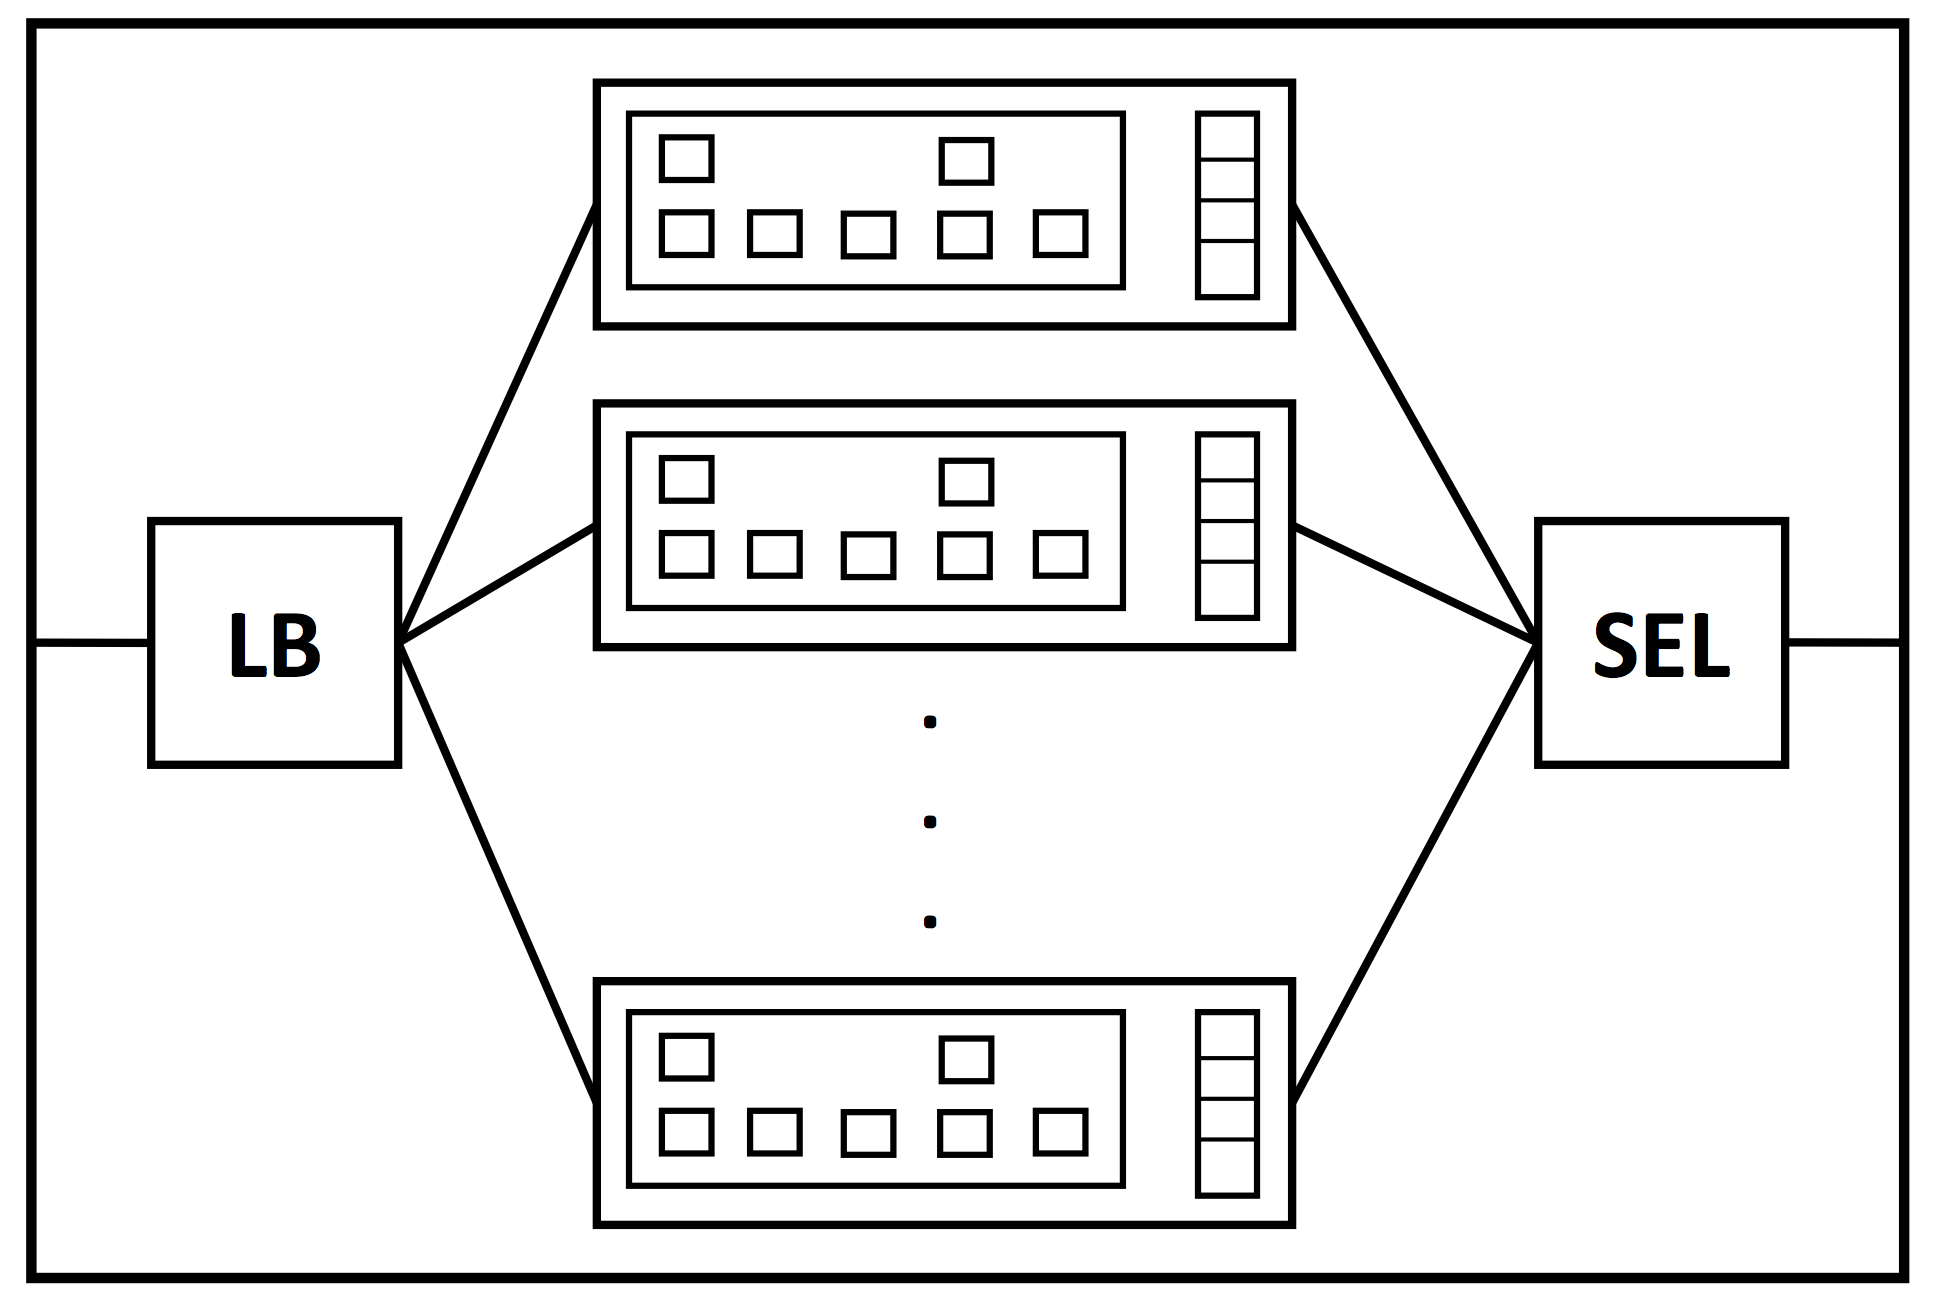
\includegraphics[width=0.8\linewidth]{figures/design/pifo-top}
\caption{Top level PIFO block diagram. LB is the enqueue load balancing module and SEL is the dequeue selector module.}
\label{fig:pifo-top}
\end{figure}

\begin{figure}[!ht]
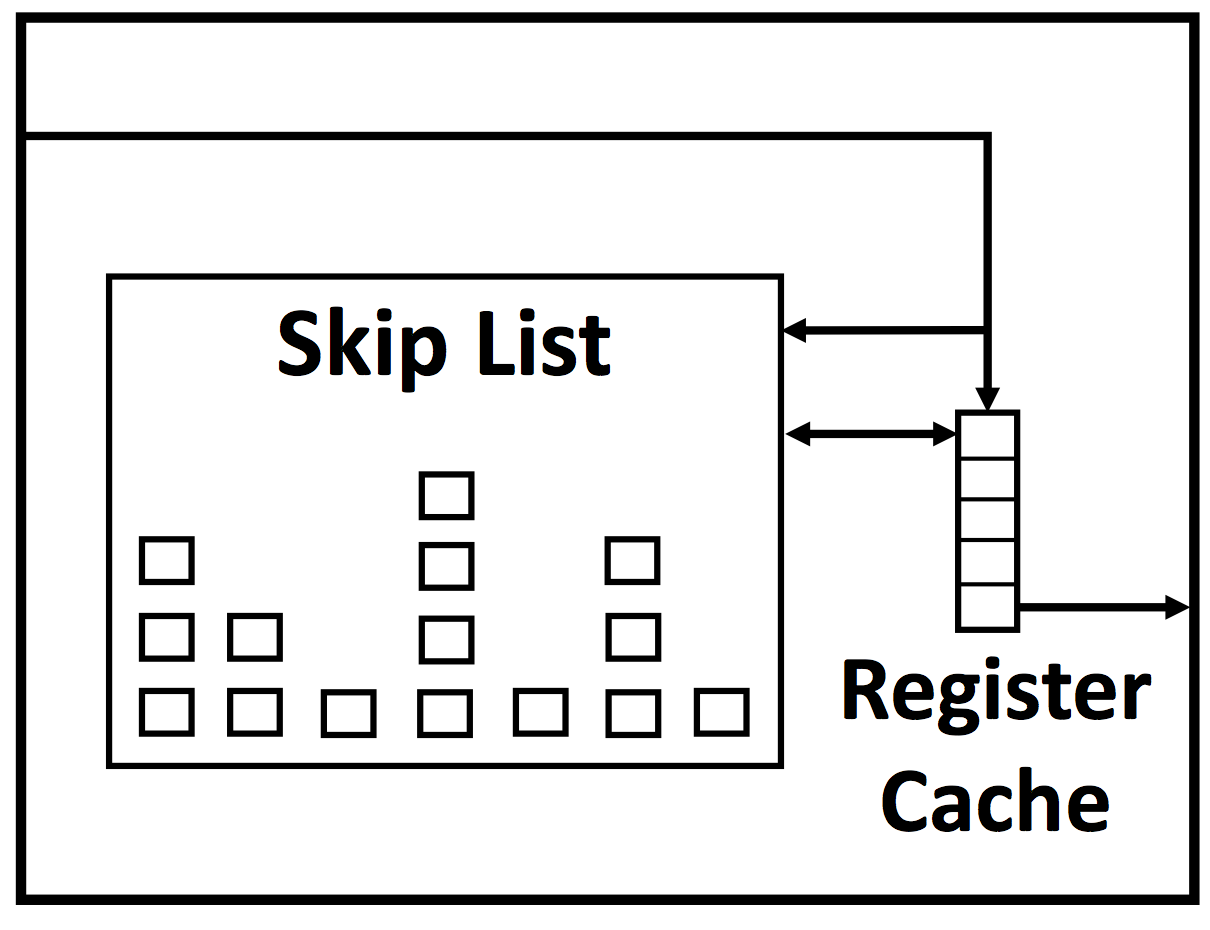
\includegraphics[width=0.7\linewidth]{figures/design/priority-queue}
\caption{Priority queue block diagram}
\label{fig:priority-queue}
\end{figure}

\subsection{Priority Queue}\label{sec:priority-queue}

The priority queue that we have designed is in fact a PIFO that can be drained at line rate and filled at sub-line rate. It sorts packet descriptors in the order of decreasing rank values. Figure \ref{fig:priority-queue} shows the top level priority queue which is composed of a register-based cache and a skip list. Each of these components is explained in more detail in sections \ref{sec:reg-cache} and \ref{sec:skip-list-impl}, respectively. Once again, the register cache and the skip list are both PIFOs, each with different enqueue and dequeue properties. The size of the cache is on the order of $log_2$ the size of the skip list and can support one enqueue and one dequeue every other cycle. The latency for an enqueue operation into the skip list is also logarithmic in the number of packet descriptors that are currently in the skip list. It typically takes one or two orders of magnitude longer than an enqueue into the cache for a skip list with a fill level of approximately 2000 packet descriptors. A dequeue from the skip list is also affected by its current size, but it is typically much faster than an enqueue. Furthermore, in order to maintain a simple skip list implementation, the design serializes enqueue and dequeue operations for the skip list.

%\todo[inline]{Explain requirements for line rate performance. Don't let output register drain. How do we guarantee this?}

% Algorithm~\ref{alg:enq-proc} describes the procedure for inserting an element into the priority queue...

%Algorithm~\ref{alg:busy-proc} describes the procedure for generating the priority queue's busy signal, which prevents the top level PIFO from attempting to enqueue anything into the priority queue...

%It could be the case that a single priority queue receives all of the smallest ranks... requires a single priority queue to drain at line rate.


%\begin{algorithm}
%\footnotesize
%\caption{Priority Queue Busy Signal Generation}\label{alg:busy-proc}
%\begin{algorithmic}[1]
%  \If{$skip\_list.busy$}
%    \State $busy = 1$
%  \Else
%    \State // $skip\_list.enq\_delay$ measured in increments of 12.8 cycles
%    \If{$skip\_list.enq\_delay > out\_reg.size$}
%      \State $busy = 1$
%    \Else
%      \State $busy = 0$
%    \EndIf
%  \EndIf
%\end{algorithmic}
%\end{algorithm}


\subsection{Fast Register-based Cache}\label{sec:reg-cache}

We use a small cache implemented using registers to significantly reduce the average enqueue and dequeue times.  The packet ranks stored in the cache are not ordered and the cache continuously advertises the minimum and maximum ranks stored in it. If the cache is full, when a new value is enqueued, it is compared with the maximum rank in the cache and then inserted in the skip list (when the new value is larger) or in the cache replacing the maximum value, which is sent to the skip list (when the new value is smaller). The cache insertion logic is shown in Algorithm \ref{alg:enq-proc}.

\begin{algorithm}
\footnotesize
\caption{Cache Insertion Procedure}\label{alg:enq-proc}
\begin{algorithmic}[1]
  \State \underline{For every arriving packet: $p$}
  \If{$cache.size < cache.max\_size \And skip\_list.size = 0$}
   \State $cache.insert(p)$
  \Else 
    \If{$p.rank < cache.max\_rank$}
     \State $skip\_list.insert(cache.max\_rank)$
     \State $cache.insert(p)$
    \Else
     \State $skip\_list.insert(p)$
    \EndIf
  \EndIf
\end{algorithmic}
\end{algorithm}

The cache is sized to hold at least $log_2$ the number of elements that can be stored in the skip list.  This size accommodates the fill level required for the starvation prevention mechanism mentioned in section \ref{sec:add-features}.

\subsection{Skip List}\label{sec:skip-list-impl}

The key to implementing a scalable PIFO is to find an appropriate data structure that facilitates simple insertion operations and fast in-order removal operations.

The skip list was first described in 1990~\cite{skip-list-1990} as a probabilistic alternative to balanced trees. They are attractive because of their simple implementation and fast insert and remove operations, which, on average, take logarithmic running time in $n$, the number of elements. The probabilistic nature of skip lists, however, means that the worst-case performance is unbounded. This is unacceptable because we require guaranteed line rate performance with our PIFO. 

Deterministic skip lists~\cite{det-skip-list} retain the simple implementation details of their probabilistic counterparts, while bounding the insertion and removal operations to functions of $\log n$. They are able to achieve this by enforcing a few simple rules upon insertion and removal to ensure that the skip list maintains a regular structure that bounds the worst-case insertion and removal times. Figure \ref{fig:skip-list-a} shows an example 1-2-3 skip list and the path that would be taken to insert element 29 into the data structure. The insertion operation always starts at the top level's tail element. It then skips across the top level until seeing that the next element is less than or equal to the value being inserted at which point it drops down a level. This process continues until reaching the insertion position in the bottom level. The 1-2-3 skip list structure policy enforces that there are no more than three consecutive nodes at the same level. Therefore, since our insertion operation caused the skip list to violate this structure requirement, we must add a level to node 18 in the third level and to node 26 in the second level. The resulting skip list is shown in Figure \ref{fig:skip-list-b}.
\paragraph{Worst-case insertion time} 
In a 1-2-3 skip list with $L$ levels, the worst-case insertion time occurs when three consecutive nodes are encountered at each level, requiring the addition of a node at each level.  
The operations that are performed are: 
\begin{itemize}
\item At each level:
\begin{itemize}
\item 3 node reads
\item 1 balancing node insertion
\end{itemize}
\item 1 new node insertion
\end{itemize}
Each node insertion requires two write operations, one for the node being added and one for the neighboring node or nodes\footnote{Multiple nodes can be written simultaneously as described in section \ref{sec:add-features} }.
The worst-case insertion time is given by
\begin{equation}\label{worst-case-insert_eqn}
(3 T_{Rd} + 2 T_{Wr} + K_{1}) (L - 1) + 2 T_{Wr} + K_{2}
\end{equation}
where:\\
\indent $T_{Rd}$ = node read time\\
\indent $T_{Wr}$ = node write time\\
\indent $K_{1}$, $K_{2}$ = processing overhead\\

\begin{figure*}[t!] % "[t!]" placement specifier just for this example
\centering
\begin{subfigure}{\linewidth}
\centering
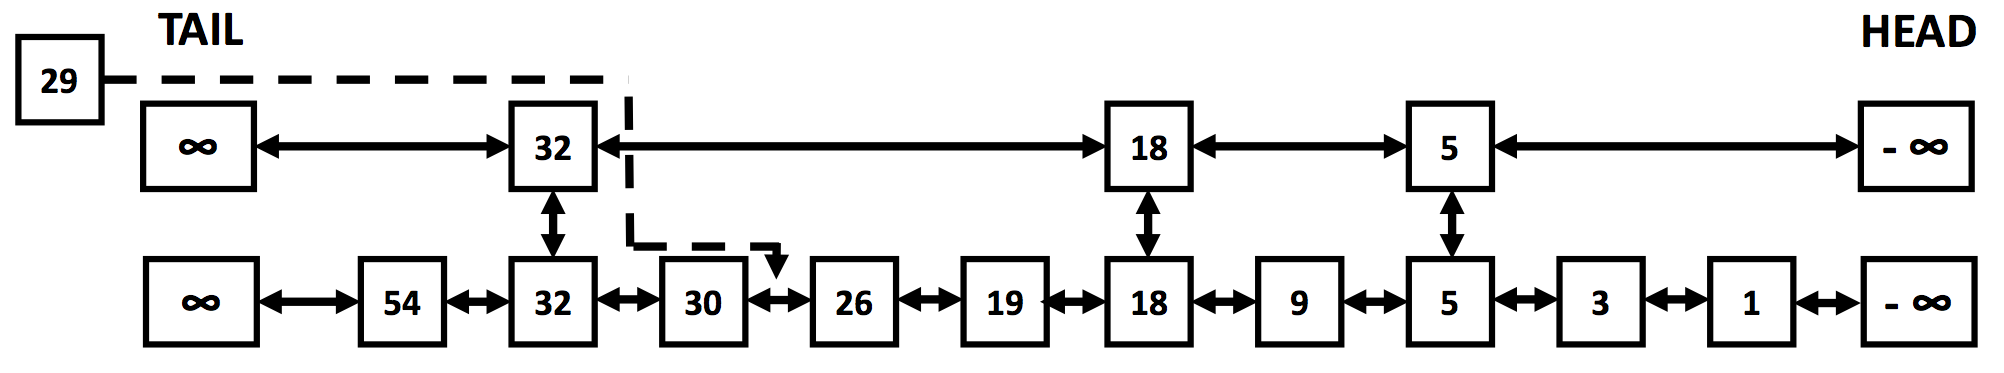
\includegraphics[width=0.8\linewidth]{figures/design/skip-list-a}
\caption{Original 1-2-3 skip list and the path to insert element 29.} \label{fig:skip-list-a}
\end{subfigure}\hspace*{\fill}

\medskip
\begin{subfigure}{\linewidth}
\centering
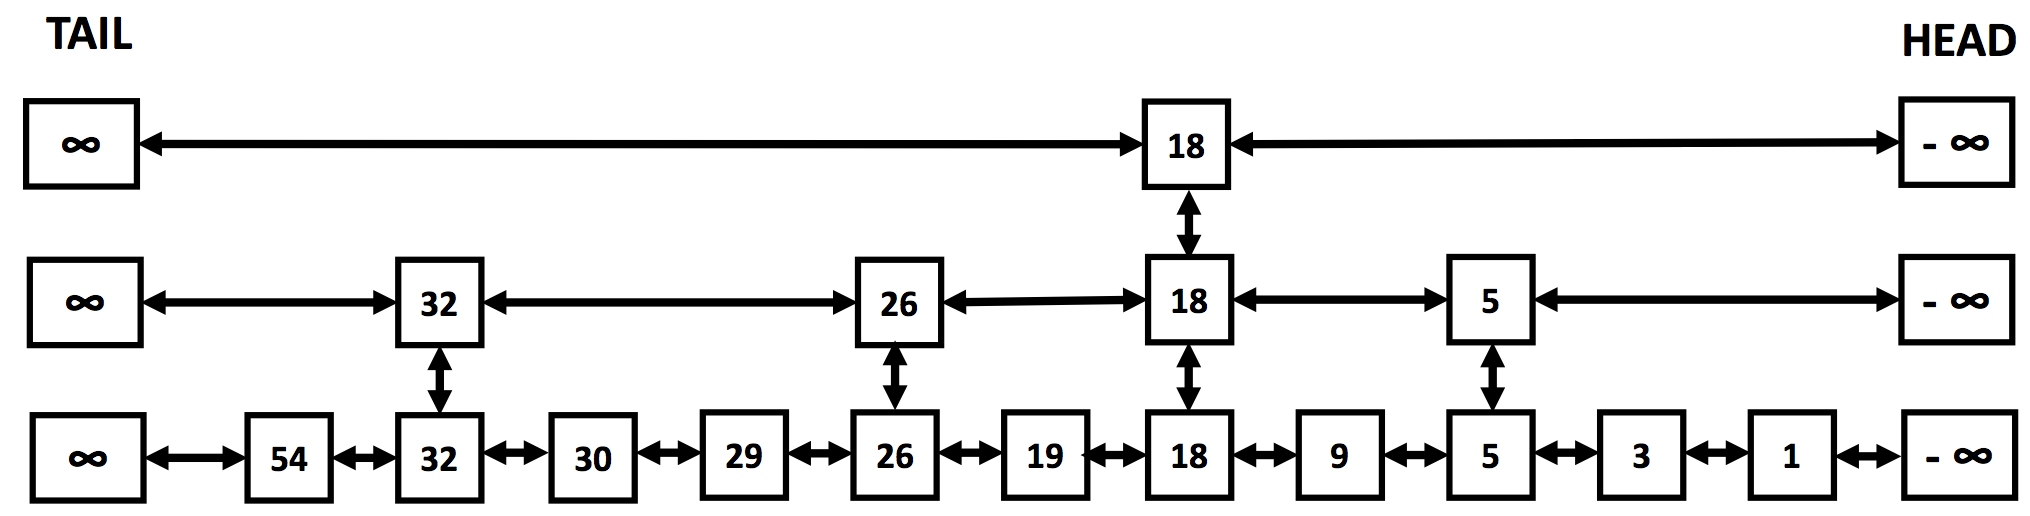
\includegraphics[width=0.8\linewidth]{figures/design/skip-list-b}
\caption{Final 1-2-3 skip list after inserting element 29.} \label{fig:skip-list-b}
\end{subfigure}\hspace*{\fill}

\caption{Insertion into a 1-2-3 deterministic skip list.}\label{fig:skip-list}
\vspace{-1.0em}
\end{figure*}

The astute reader will recall that elements are always dequeued from the head of a PIFO. This means that if we use a skip list as the underlying primitive with which to implement a PIFO then the removal operation becomes trivial, simply remove the head element.  There is no complicated re-balancing logic that must take place.

\subsubsection{Additional Design Features}\label{sec:add-features}
The following design features were used to improve performance
\paragraph{Skip List Pointers}
A standard skip list uses two pointers:
\begin{itemize}
\item A $right$ pointer to move forward from the tail towards the head
\item A $down$ pointer to move from any level to the base level
\end{itemize}
We added two pointers, $left$ and $up$ to speed up the dequeue operation, including freeing nodes from upper levels if any.

Since every enqueue operation starts by reading the tail node at the top level and every dequeue by reading the head node at the bottom level, we store these pointers in registers to eliminate a block RAM access.

In addition, we used separate memories for each of the four pointers, which allows us to update different pointers for different nodes in a single clock cycle.  For example, when adding a new node for balancing, pointers on the left, right, and down neighboring nodes are updated in a single clock cycle.

\paragraph{Enqueue Throttling}\label{enq-throttle}
As locations in the cache become vacant due to dequeues, they are replenished from the head of the skip list as a background process.  If a cache insertion and a removal coincide, the insertion takes precedence and the replenishment of the cache is delayed.  To prevent cache starvation under high enqueue rates, we introduced an enqueue throttling mechanism that maintains a cache fill level such that the cache will not become empty if the replenishment is blocked for a worst-case enqueue time.  

The throttling is activated using a dynamic threshold that is a function of the fill level of the skip list.  The net effect is that the fill level of the cache varies with the fill level of the skip list; if the skip list is more full, enqueue time is longer and therefore we need more descriptors in the cache to maintain the dequeue rate.  The enqueue throttling allows sustained dequeuing from a single priority queue every four clock cycles while not adversely affecting the enqueue latency. We have used the following thresholds for controlling the cache fill level as a function of the skip list fill level (up to 2048 descriptors).

\begin{center}
\begin{tabular}{|c|c|}
    \hline
    \textbf{Skip List Fill Level} & \textbf{Cache Fill Level} \\
    \hline
    0 & 0\\
    \hline
    1 & 1\\
    \hline
    2 - 3 & 2\\
    \hline
    4 - 7 & 3\\
    \hline
    8 - 15 & 4\\
    \hline
    16 - 31 & 5\\
    \hline
    32 - 63 & 6\\
    \hline
    64 - 127 & 7\\
    \hline
    128 - 255 & 8\\
    \hline
    256 - 511 & 9\\
    \hline
    512 - 1023 & 10\\
    \hline
    1024 - 2047 & 11\\
    \hline
\end{tabular}
\end{center}

It is not surprising that the cache fill level is a logarithmic function of the skip list fill level, since the skip list enqueue time is also a logarithmic function of the fill level.

\subsection{Multi-Port Scheduler Design}\label{sec:sched-des}

This section describes how to build a multi-port scheduler utilizing the line rate PIFO design described in the previous sections. We propose to use a virtual output PIFO queuing architecture. This means that each PIFO must support both insertions and removals at line rate in order to sustain the worst case traffic patterns. 

%\subsubsection{NetFPGA Platform}

%The NetFPGA SUME is a {4x10Gb/s} networking hardware platform that provides programmability via a Virtex-7 FPGA. The NetFPGA reference design runs at a core clock frequency of 200 MHz using a 256-bit datapath; fast enough to support more than 40Gb/s. Figure XXX shows a block diagram of how we integrated our scheduler into the NetFPGA reference design. The reference design that we used consists of four input ports and four output ports, each running at 10Gb/s. An input arbiter performing deficit round robin scheduling reads packets out of the input queues and injects them into the core datapath. The output port lookup module is responsible for deciding the packet's destination port, rank, and queue ID. These three decisions are passed along with the packet to our scheduling block, which then makes the appropriate scheduling decision and forwards packets to appropriate the output port.

%\todo[inline]{insert NetFPGA reference design with scheduler.}

\subsubsection{Top Level Scheduler Design}\label{sec:top-level-sched}

Figure \ref{fig:tm-top} shows a block diagram of our top level scheduler design. The design uses a virtual output PIFO queuing architecture, such that there is one PIFO for each output port at each of the input ports. Each input port also has a partition of packet buffer storage which is shared amongst all of the PIFOs at that port. Full packets are stored in the packet buffer and packet descriptors are enqueued into and scheduled by the PIFOs. Assuming that packets are not broadcast or multicast, the packet buffer as well as each PIFO must be fast enough to perform both enqueue operations and dequeue operations at exactly line rate, or 10Gb/s for our design. The line rate and clock frequency directly dictate the maximum number of clock cycles alloted to process each packet in order to guarantee line rate performance. Our design uses a 200 MHz clock, which means that the maximum number of clock cycles to process each packet is determined by the following equation,

$$ \frac{(8~B + 64~B + 12~B)\times 200~MHz}{10~Gb/s} = 13.44~\mbox{cycles} $$

This assumes the minimum size packet is 64B and there is an 8B preamble and Start of Frame Delimiter and a 12B interframe gap. The above result enforces a hard constraint on the design of our PIFO which must be able to both enqueue and dequeue a packet descriptor once every 13.44 cycles. Additionally, the packet buffer must be able to enqueue and dequeue 64B packets every 13.44 cycles. 

In addition to the PIFO and packet buffer, the design also consists of a PIFO selector module at each output port. This module is responsible for comparing the rank values at the head of its corresponding virtual output PIFOs to decide which packet to transfer into the output queue. The selector will dequeue the packet with the smallest rank. Each packet descriptor is also accompanied by an enqueue timestamp, which is used to break ties in cases where there are identical ranks across virtual output PIFOs. This timestamp allows the scheduler to guarantee that packets configured with the same rank depart in FIFO order.


\begin{figure}[!h]
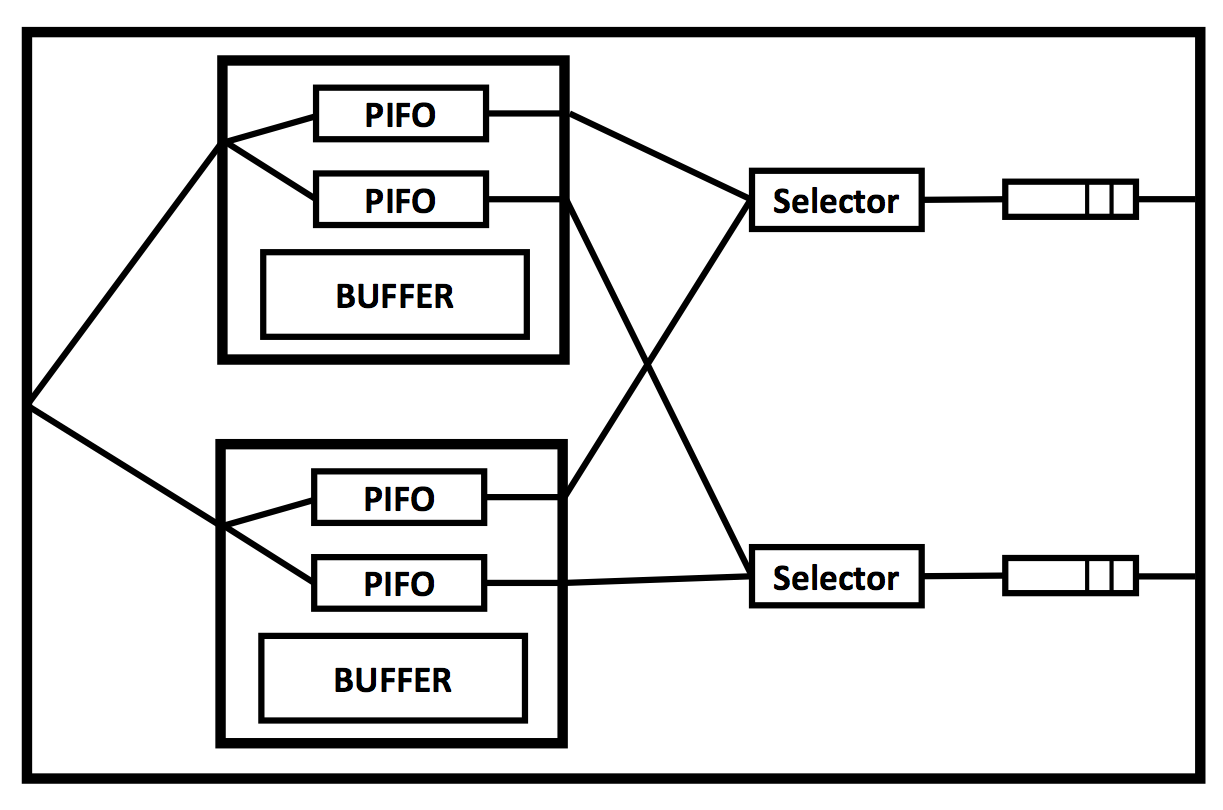
\includegraphics[width=1\linewidth]{figures/design/tm-top}
\caption{Top level traffic manager}
\label{fig:tm-top}
\end{figure}

\subsubsection{Packet Buffer}

The packet buffer consists of two BRAM modules, one to store 64B packet segments and another to store packet metadata. Unoccupied metadata slots and packet segments are accounted for using free lists. Packet segments are connected using a singly linked list.

Each input port is configured to have 130KB of packet segment storage (2048 segments); enough for about 100us of buffering, which is a typical RTT in datacenter networks~\cite{timely}. The packet buffer is designed to be the limiting resource at each input port. In other words, there will always be enough room in the PIFOs to store packet descriptors. Network operators often want to partition the available buffer space into some number of queues. These queues are used to isolate different classes of traffic, such that one does not consume the buffer space of another. In our design, the number of queues and their sizes are fully configurable. Queue sizes are enforced using simple counters which track the number of packet segments currently being consumed by each queue. Our design implements the tail drop policy; if a packet arrives destined for queue $N$ and the counter for queue $N$ has reached its maximum configured value then the packet is dropped.

While the design currently uses a static partitioning of buffer space into queues, in practice, this allocation would like be dynamic. This would simply require updating the control registers that are used to configure the queue allocations in our design. Furthermore, large FPGA memories or external RAM can be used to increase the size of the packet buffer.


%%%%%%%%%%%%%%%%%%%%%%

%%%%%%%%%%%%%%%%%%%%%%
%%%%%%%%%%%%%%%%%%%%%%
\section{Evaluation}
%%%%%%%%%%%%%%%%%%%%%%

In this section, we profile various aspects of our PIFO design to justify our design choices and demonstrate its capability to achieve line rate performance. We use a  200MHz reference clock in these evaluations.

\subsection{Priority Queue Evaluation}

As explained in Section~\ref{sec:priority-queue}, the priority queue consists of a single skip list and a cache. It is designed to satisfy two properties:
\begin{enumerate}
  \item Packet descriptors can be enqueued at less than line rate
  \item Packet descriptors can be dequeued from the head at line rate
\end{enumerate}

The following sections describe experiments that allow us to characterize the enqueue and dequeue performance of a single priority queue.

\subsubsection*{Effect of Fill Level}
Descriptors can be enqueued into the cache every other clock cycle. The main factor that drives the rate at which descriptors can be enqueued into the skip list is the number of memory operations that are required to find the appropriate insertion location, which increases logarithmically with the number of the descriptors in the skip list. We define the fill level as the number of descriptors in both the skip list and the cache.

Figure \ref{fig:fill_level} shows the effect of the fill level on both the enqueue and the dequeue latency, that is, the number of clock cycles required to complete each of these operations. This experiment uses a skip list with a capacity of 2048 elements (using 12 levels) and 16- entry cache. Each average and maximum is computed over 100 samples. As expected, the enqueue latency increases logarithmically with the number of descriptors and the maximum possible enqueue latency is 130 clock cycles, which agrees with the theoretical maximum given by equation \ref{worst-case-insert_eqn}, with $L = 12$, $T_{Rd}$ = 2, $T_{Wr}$ = 1, $K_{1}$ = 3, and $K_{2}$ = 7.

This result constrains two additional aspects of the design:
\begin{enumerate}
  \item The minimum size of the output register to ensure that it has enough capacity to avoid running empty during the longest possible enqueue operation into the skip list.
    \item The number of priority queues that must be used in parallel in order to support enqueue operations at line rate.
\end{enumerate}

All packets used in this experiment are 64B in length, which take 2 cycles to transfer using our 32B data-path. The dequeue latency plot shows that these 64B packets can be removed in three to five cycles depending on whether the dequeue operation is directly preceded by an insertion into the register cache. This is more than fast enough to meet our 13.44 cycle deadline for 10Gb/s operation.

\begin{figure}[!h]
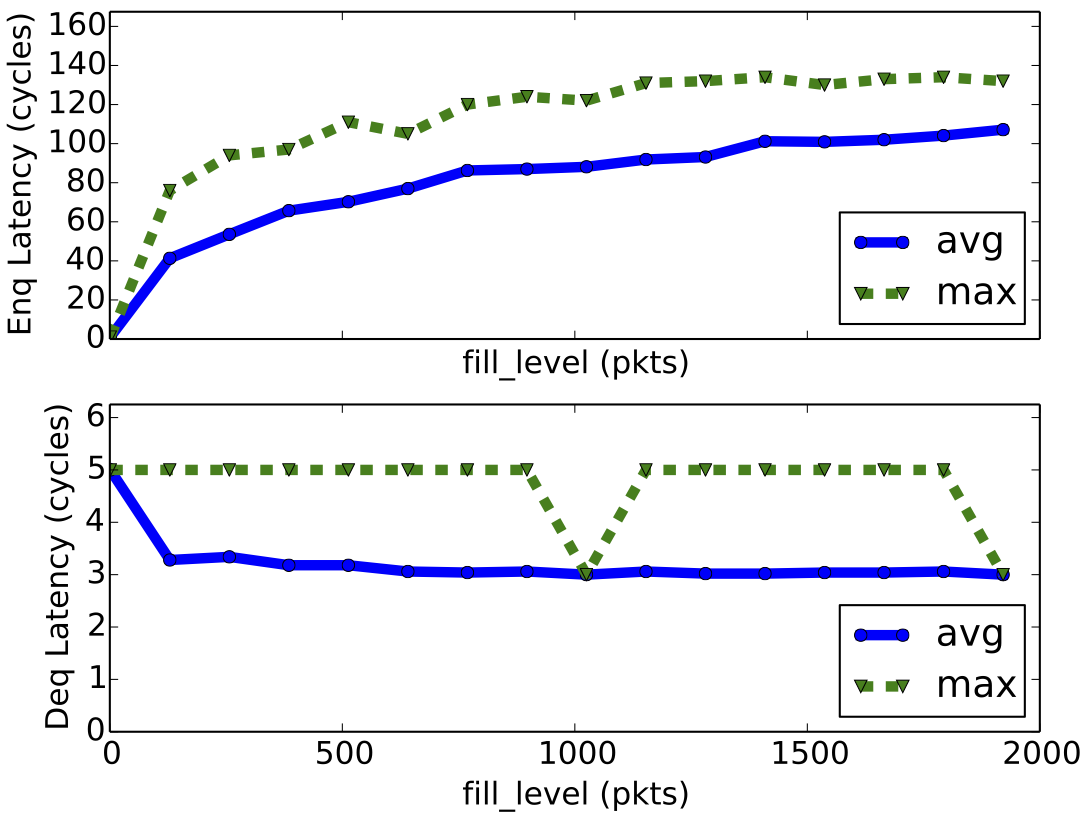
\includegraphics[width=1\linewidth]{figures/eval/enq_deq_v_fill_level}
\caption{Effect on the enqueue and dequeue latencies when the number of entries in the priority queue increases.}
\label{fig:fill_level}
\end{figure}

\subsubsection*{Sizing the Output Register}
The output register must be large enough to satisfy two constraints:
\begin{enumerate}
  \item Large enough to absorb the variations in the rate at which it is being filled by the background process that is replenishing it with descriptors from the skip list.
  \item Large enough to be able to hold enough descriptors such that it will not run empty when the longest possible skip list insertion begins and replenishment from the skip list temporarily stops.
\end{enumerate}

Both of these conditions must be met in order to guarantee that the scheduler will remain work conserving under all conditions. 

To satisfy the first constraint, we must be able to bound the rate at which descriptors are dequeued from the skip list and inserted into the output register. Fortunately, the deterministic structure of the skip list allows us to do exactly that. The maximum number of clock cycles required to dequeue an element from the head of the skip list is directly related to the number of levels in which the head element is present ($L$). This relationship is given by the following expression,

\begin{equation}\label{worst-case-remove_eqn}
T_{Rd} \times L + K_{3}
\end{equation}
where:\\
\indent $T_{Rd}$ = node read time\footnote{Writes are performed as well but they do not contribute to the latency because they are performed in parallel with the reads} = 2 clock cycles\\
\indent $K_{3}$ = processing overhead = 6 clock cycles\\

The deterministic skip list structure property enforces that the node heights, i.e. the number of levels in which they appear, are well distributed. This means that the dequeue rate from the skip list is mostly constant. Figure \ref{fig:out_reg_size} shows the fill level of the output register during an experiment where the skip list starts out filled with 2K descriptors and is then drained at a rate of one descriptor every 12 cycles, faster than line rate. We see that the number of descriptors in the output register never drops by more than two indicating that it is indeed being filled faster than it is being drained. Our measurements indicate that on average, the head element can be removed from the skip list in 8 cycles and in the worst case it can take up to 30 cycles, just over two minimum packet times.

\begin{figure}[!ht]
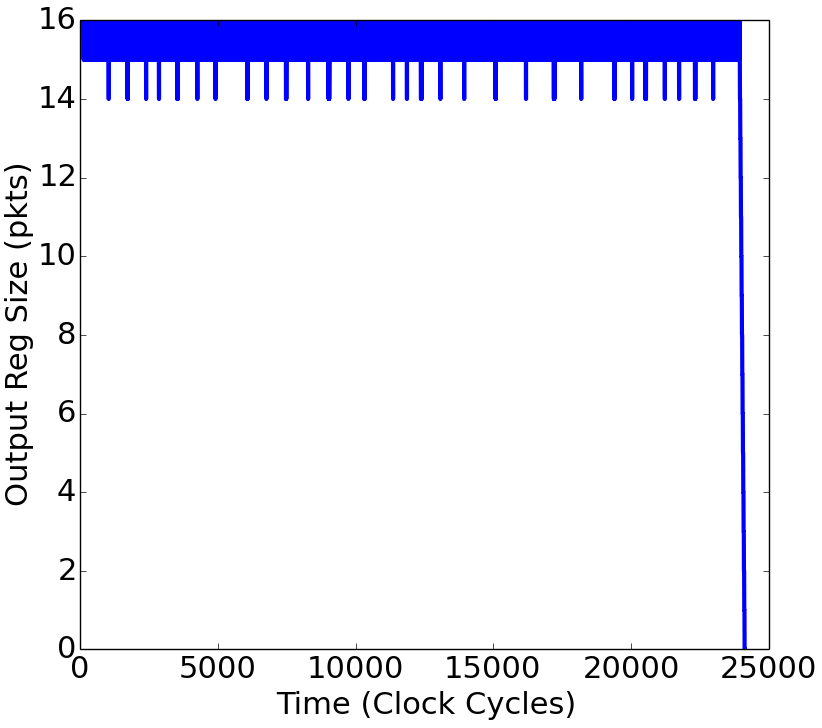
\includegraphics[width=1\linewidth]{figures/eval/out_reg_size}
\caption{The fill level of the output register while draining a skip list with 2K descriptors.}
\label{fig:out_reg_size}
\end{figure}

The output register must also be large enough to avoid going empty during a long skip list enqueue operation. This turns out to be a tighter constraint than (1) because an enqueue into the skip list can last up to 130 cycles. The output register will be drained at line rate of up to one descriptor every 13.44 cycles. This means than it must be able to hold at least 10 descriptors in order to sustain line rate without missing any dead lines.

\subsection{PIFO Evaluation}

A single priority queue cannot support enqueue operations at line rate. This is why a PIFO is composed of multiple priority queues combined in parallel and the enqueue operations are load balanced across all of them. The following section describes the results of the experiment we used to analyze the relationship between the enqueue latency and the number of parallel priority queues.

\subsubsection*{Number of parallel priority queues}
We conducted multiple experiments varying the number of parallel priority queues and use a fill level of 2000 packets. We report the average and maximum enqueue latency over 100 samples for each experiment. Figure \ref{fig:num_skip_lists} shows that the enqueue latency is very sensitive to the number of priority queues that are used in parallel. As the number of priority queues increases, the fill level of each one decreases and hence enqueue operations complete more quickly. This results in an inverse log relationship between enqueue latency and number of priority queues. We find that the design must use at least 11 parallel skip lists to support line rate enqueue operations, that is, one enqueue every 13.44 cycles. Figure \ref{fig:num_skip_lists} also shows that the dequeue latency is well under this 13.44 cycle requirement as well.

\begin{figure}[!h]
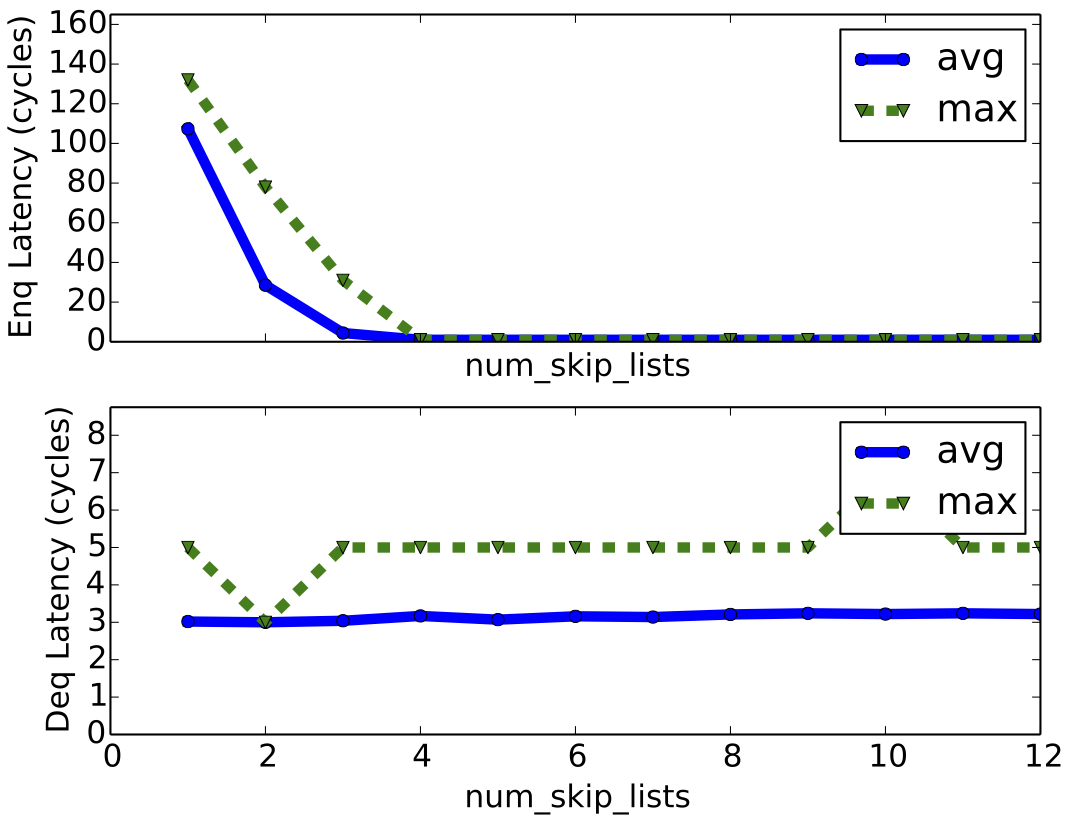
\includegraphics[width=1\linewidth]{figures/eval/enq_deq_v_num_skip_lists}
\caption{Effect of using more parallel skip lists on the enqueue and dequeue latencies.}
\label{fig:num_skip_lists}
\end{figure}


\subsubsection*{Utilization Summary}
We compiled our PIFO onto a Virtex-7 FPGA in order to calculate the resource utilization and verify that the design meets all timing constraints. Table \ref{tab:utilization} provides a summary of the FPGA resource utilization for a single PIFO.

\begin{table}[tbp]
\centering
\caption{Virtex-7 resource utilization for a single PIFO that uses 11 parallel priority queues and has a total capacity of 2K packet descriptors.}
\label{tab:utilization}
\begin{tabular}{|l|l|}
\hline
\multicolumn{1}{|c|}{\textbf{Resource}} & \multicolumn{1}{c|}{\textbf{Utilization}} \\ \hline
LUTs                                    &  51777                                         \\ \hline
FFs                                     &  40586                                         \\ \hline
32Kbit BRAM Tiles                       &  44                                         \\ \hline
\end{tabular}
\end{table}

\subsection{Scheduling algorithm demonstrations}\label{sec:sched-evals}

In this section, we provide the first demonstrations of using a PIFO to implement various common scheduling algorithms. We assume that the rank computation for each scheduling algorithm has already been completed and only concern ourselves with the behavior and evaluation of the scheduling logic. The following evaluations use a single PIFO and packet buffer rather than the full scheduler design in order to minimize the required simulation time. Table \ref{tab:params} shows the design parameters that we used for these evaluations. These demonstrations indicate that our PIFO scheduler is capable of meeting line rate requirements and is flexible enough to be used as a primitive to implement common scheduling algorithms.

\begin{table}[tbp]
\centering
\caption{Parameters used for scheduling algorithm evaluations}
\label{tab:params}
\begin{tabular}{|l|l|}
\hline
\multicolumn{1}{|c|}{\textbf{Parameter}} & \multicolumn{1}{c|}{\textbf{Value}} \\ \hline
PIFO size (pkts)                         & 2048                                \\ \hline
Register Cache Size (pkts)               & 16                                  \\ \hline
Buffer size (64B segments)               & 2048                                \\ \hline
Num Skip Lists                           & 11                                  \\ \hline
\end{tabular}
\end{table}

\subsubsection*{Strict Priorities}

The strict priority scheduling algorithm guarantees that the highest priority queue receives the full egress bandwidth so long as it has any packets in it. This algorithm would be used in scenarios with a limited amount of high priority traffic. In order to implement strict priorities with a PIFO, the rank of each packet is simply equal to its assigned queue ID, where queue 0 is the highest priority queue.

We conducted an experiment where a high-bandwidth low-priority flow is combined with a short flurry of 175 high-priority packets sent at 2 Gb/s. The buffer space is partitioned into two queues and each flow is assigned to a different queue. The aggregate rate of both flows is 10 Gb/s and the PIFO is configured to drain at 4 Gb/s. Figure \ref{fig:strict_queues} shows the size of each queue for the duration of the experiment, and Figure \ref{fig:strict_rates} shows the measured input and output flow rates. We can clearly see that the high priority flow passes through the PIFO scheduler unaffected because its output rate is equal to its input rate, and the high priority queue never contains more than a single packet.

\begin{figure}[!h]
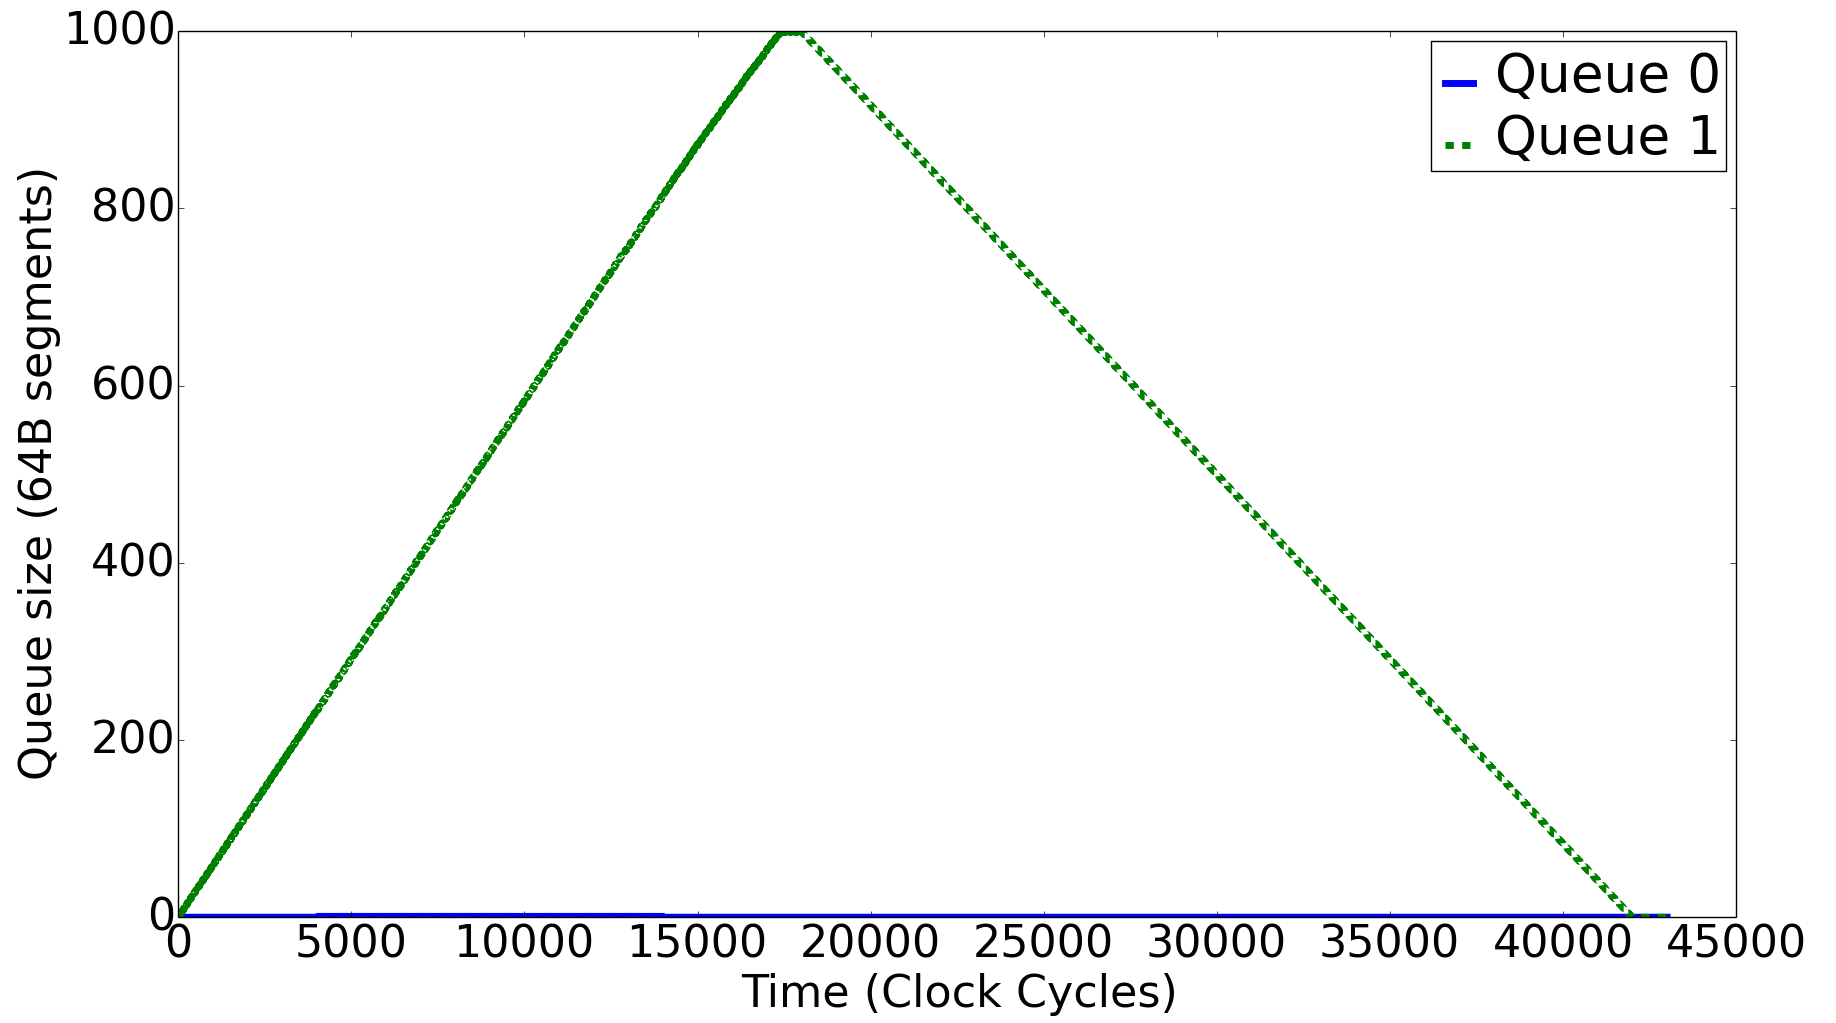
\includegraphics[width=1\linewidth]{figures/eval/strict_queues}
\caption{Queue sizes during strict priority scheduling experiment using our PIFO implementation. Queue 0 is the high priority queue.}
\label{fig:strict_queues}
\end{figure}

\begin{figure}[!h]
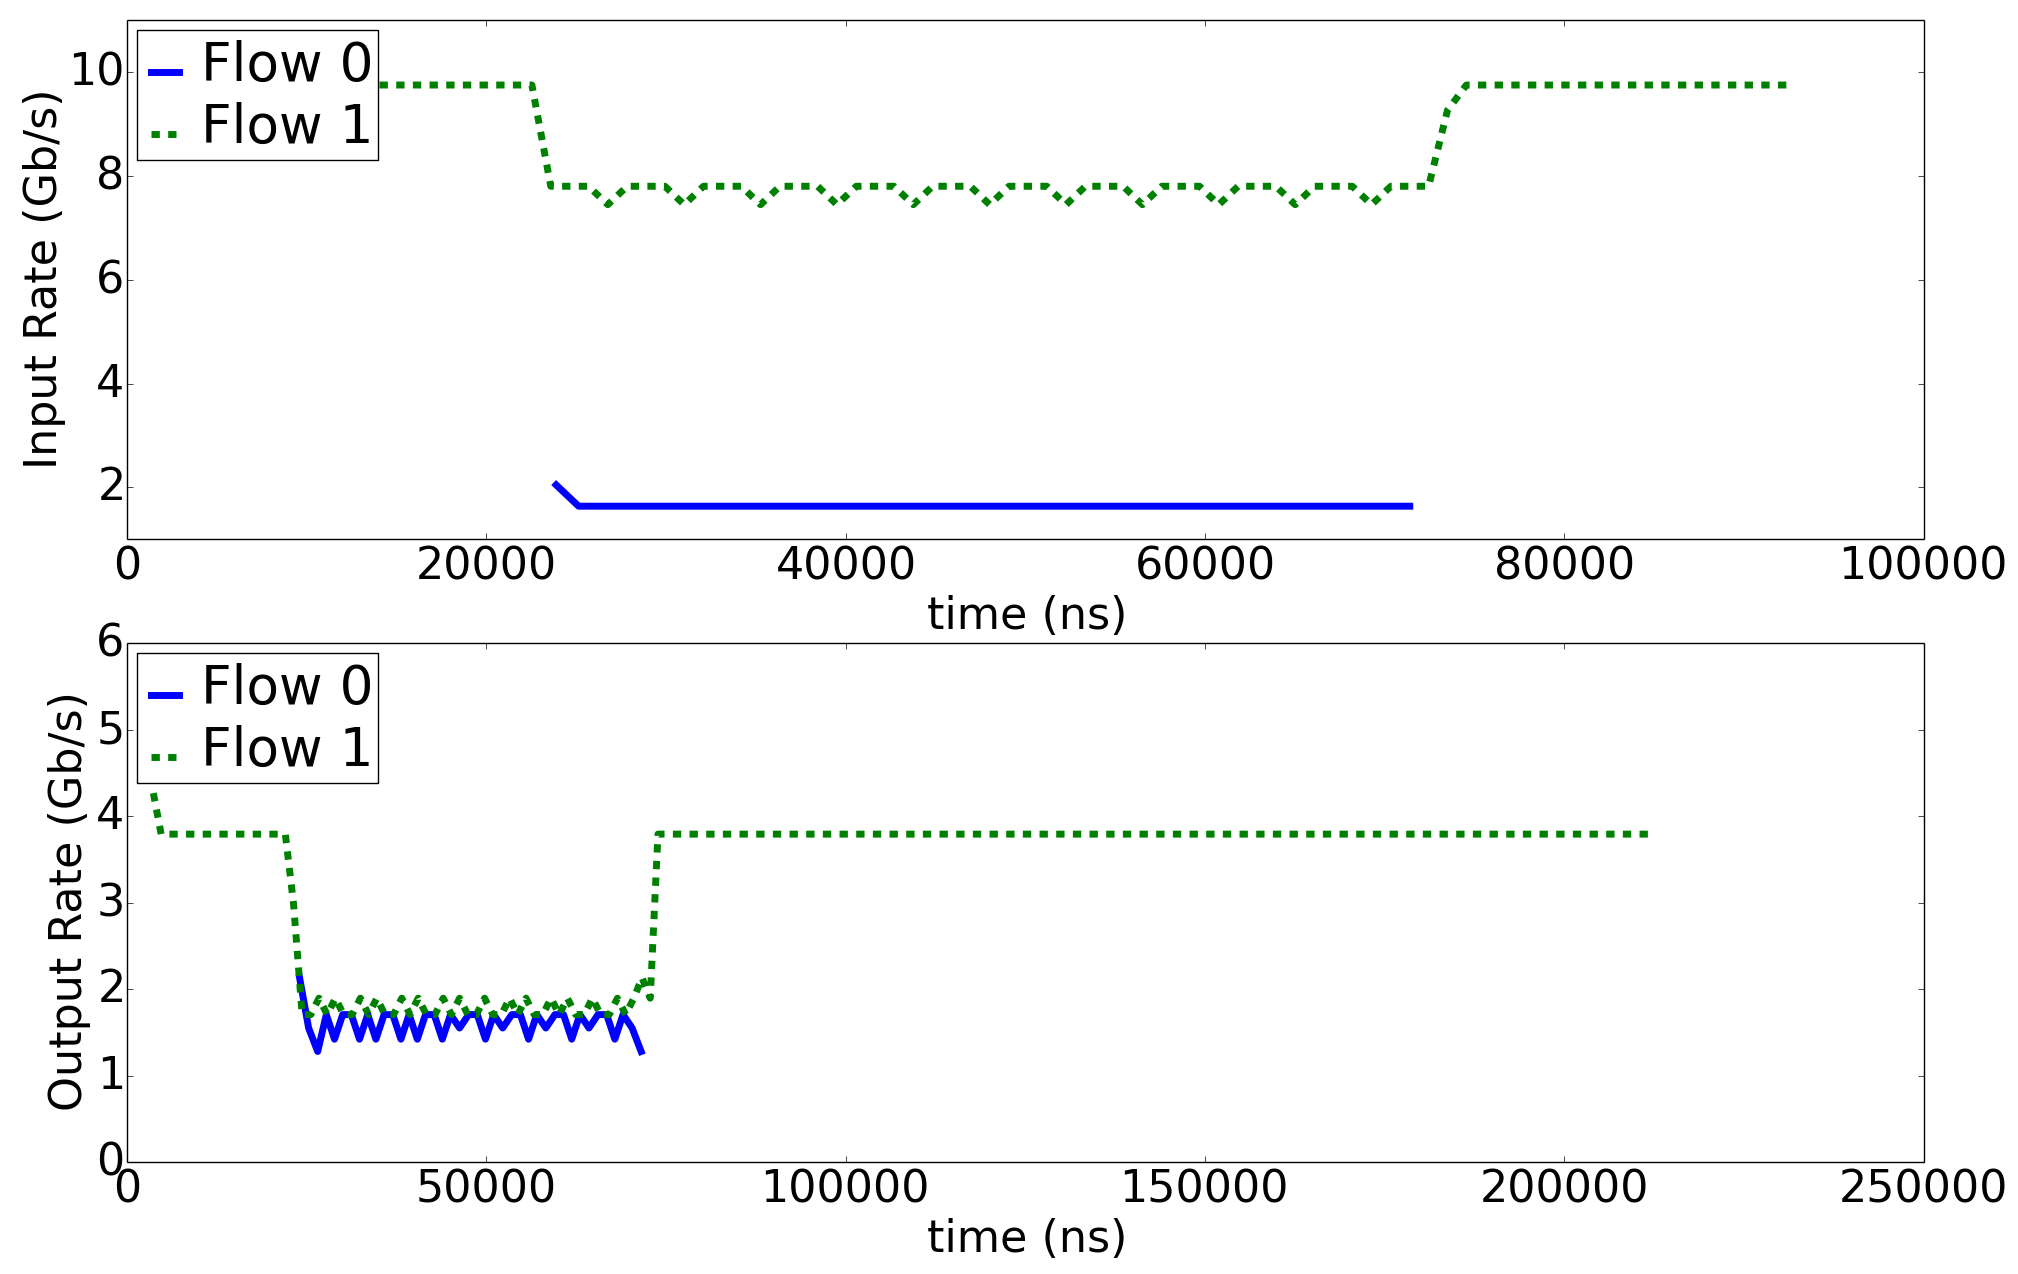
\includegraphics[width=1\linewidth]{figures/eval/strict_rates}
\caption{Strict priority scheduling using our PIFO implementation.}
\label{fig:strict_rates}
\end{figure}

\subsubsection*{Round Robin}\label{sec:round-robin}

Round robin scheduling is the process of serving a single packet from each queue in an alternating fashion. We conducted an experiment using four flows of 64B packets, where each flow has its own queue in the scheduler. The rank of each incoming packet is precomputed to implement round robin scheduling and we measured the input and output rate of each flow. The input rate of each flow is variable, but the total aggregate input rate is 10 Gb/s. The PIFO scheduler is configured to drain at 4 Gb/s. Since all packets are the same size, we would expect round robin scheduling to evenly share the egress bandwidth between all flows. Figure \ref{fig:rr_rates} shows the results of this experiment and indicates that our PIFO scheduler is indeed behaving as expected. Each of the four levels in the output rate plot indicates that the bandwidth is being equally shared between four, three, two, and one flow. The queues do not saturate during this experiment and hence there are no packet drops. This demonstrates that our PIFO scheduler is able to keep up with line rate enqueue operations.

\begin{figure}[!h]
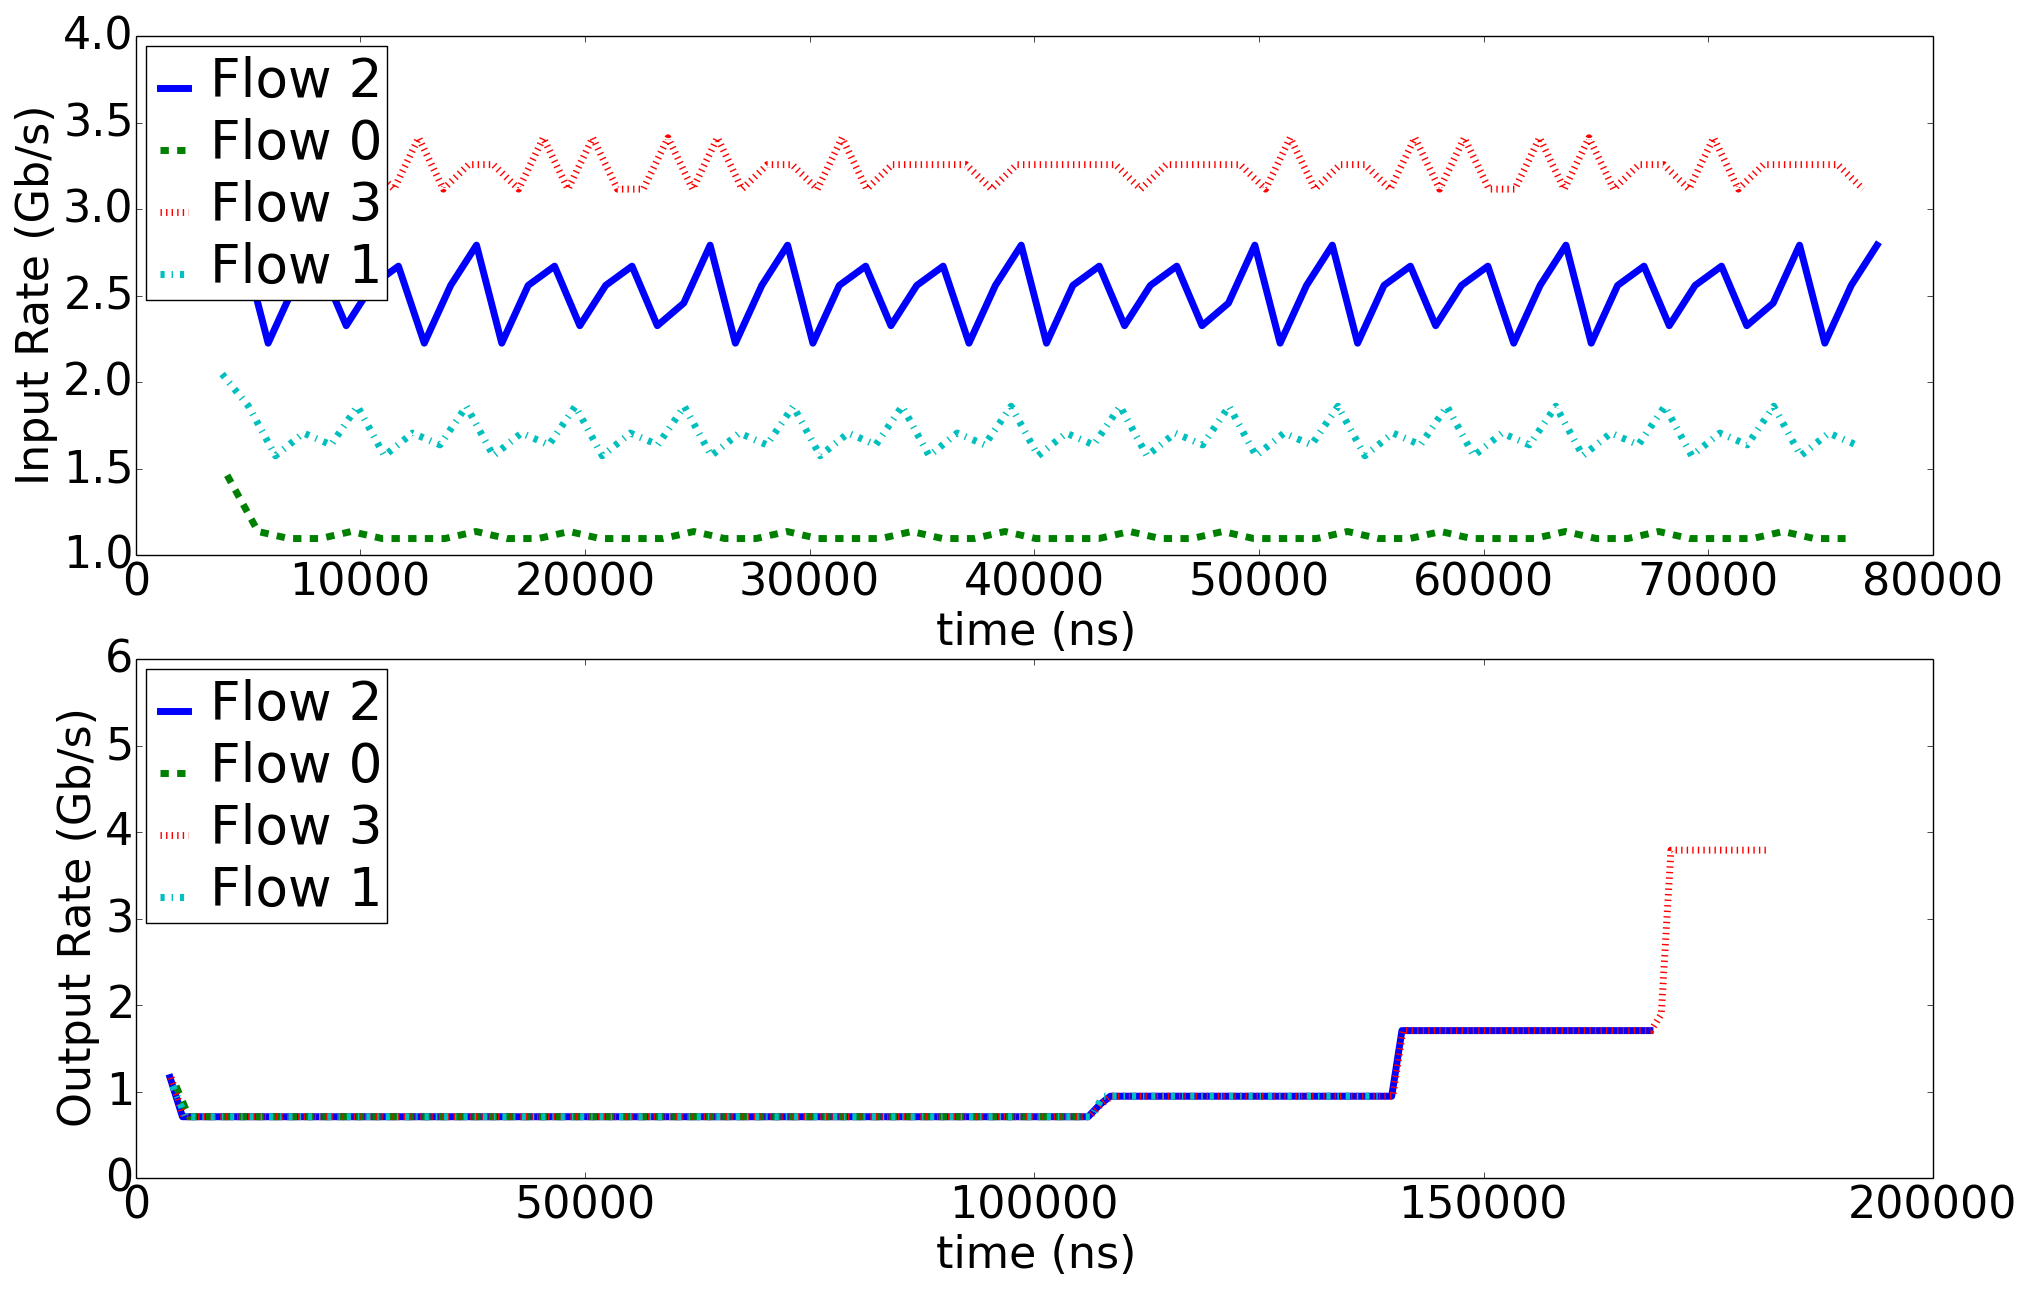
\includegraphics[width=1\linewidth]{figures/eval/rr_rates}
\caption{Round robin scheduling using our PIFO implementation. All flows are sending 64B packets.}
\label{fig:rr_rates}
\end{figure}

\subsubsection*{Weighted Round Robin}

Weighted round robin scheduling is exactly equivalent to round robin if each queue is configured with a weight of one. The queue weights can be configured such that the scheduler dequeues multiple packets from a particular queue according to its weight. We performed the same experiment as the one described in Section \ref{sec:round-robin}, except that the packet ranks are configured to assign to flow 0 a weight that is twice that of the other three flows. Figure \ref{fig:wrr_rates} shows that this weight factor allows flow 0 to pass through the PIFO scheduler completely unaffected by the other three (higher bandwidth) flows.

\begin{figure}[!h]
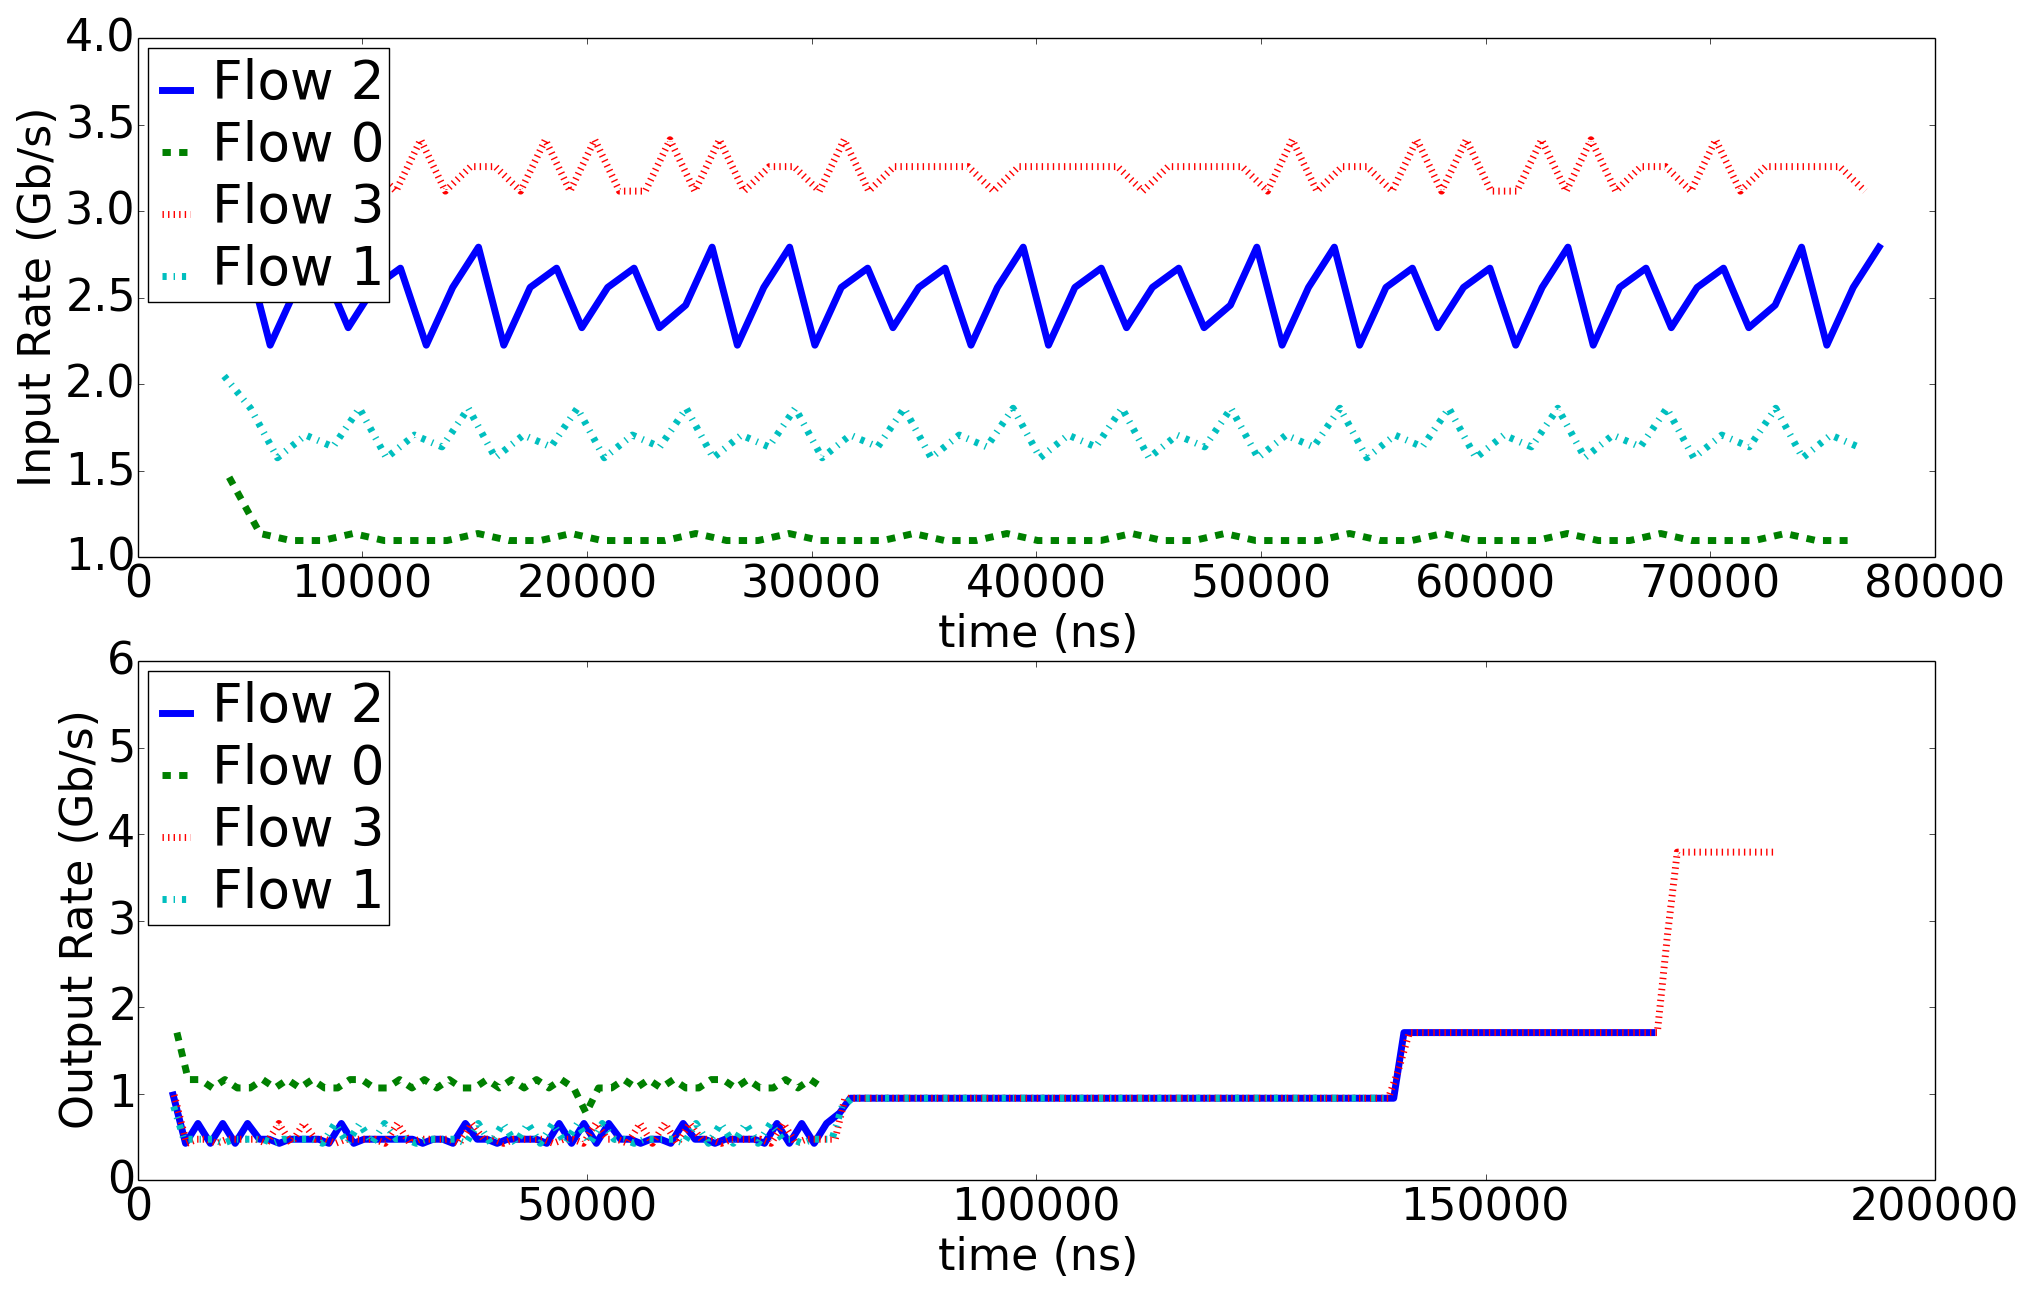
\includegraphics[width=1\linewidth]{figures/eval/wrr_rates}
\caption{Weighted round robin scheduling using our PIFO implementation. All flows are sending 64B packets. Flow 0 is weighted twice as much as the other flows.}
\label{fig:wrr_rates}
\end{figure}

% \subsubsection*{STFQ?}

% \todo[inline]{Needs some debugging}



%%%%%%%%%%%%%%%%%%%%%%

%%%%%%%%%%%%%%%%%%%%%%
%%%%%%%%%%%%%%%%%%%%%%
\section{Extensibility Discussion}
%%%%%%%%%%%%%%%%%%%%%%

\subsection{Optimizations to Current Design}\label{sec:optimizations}
The design that we propose in this paper demonstrates that it is feasible to build a 10 Gb/s line rate PIFO scheduler on an FPGA. However, we would like to point a potential optimization that would allow the design to scale to support even higher line rates.

\subsubsection*{Pipelined skip list operation}
Pipelining is the concept of partitioning logic into discrete stages to allow subsequent operations to begin processing before previous operations have fully completed. This is a common design technique that is used when designing line rate systems. For example, the authors of \cite{pipelined-heap-2007} use this approach to build a 10Gb/s pipelined heap for ASICs. The design techniques that we use in this paper, namely parallelism and a small-fast sorting cache, challenge the conventional wisdom that line rate systems must make use of heavy pipelining. Note that these techniques are completely orthogonal. We can improve the performance of our skip list implementation by pipelining the required operations. This would allow enqueue operations to occur more frequently and hence reduce the number of priority queues that must be used in parallel.

The key to building a pipelined system is to identify discrete stages of logic that perform approximately the same amount of work. For a deterministic skip list, it is natural to divide the processing of each level into individual stages. All of the nodes belonging to a particular level can be stored in a separate BRAM, as shown in Figure \ref{fig:pipe-skip-list}. Each stage then has some fixed number of clock cycles to complete the processing on the nodes in that level. Fortunately, the deterministic skip list bounds the number of memory operations that are required at each level so it is possible to fix the number of clock cycles for each stage of processing. Each level, other than the bottom, must accept search requests from the level above and insertion requests from the level below. It must also output the value it is currently searching for so that it can be immediately removed if it becomes the head element before the enqueue operation completes. The bottom level is responsible for receiving search requests from the level above, performing the initial enqueue operation, and generating insertion operations for the level above. A skip list with $N$ levels may be working on $N$ enqueue operations simultaneously. This means that a comparator must be able to examine all $N$ enqueue ranks simultaneously in order to decide which value to dequeue. Removal operations can be broadcast to all levels simultaneously along with a unique identifier for the element being dequeued.

\begin{figure}[!h]
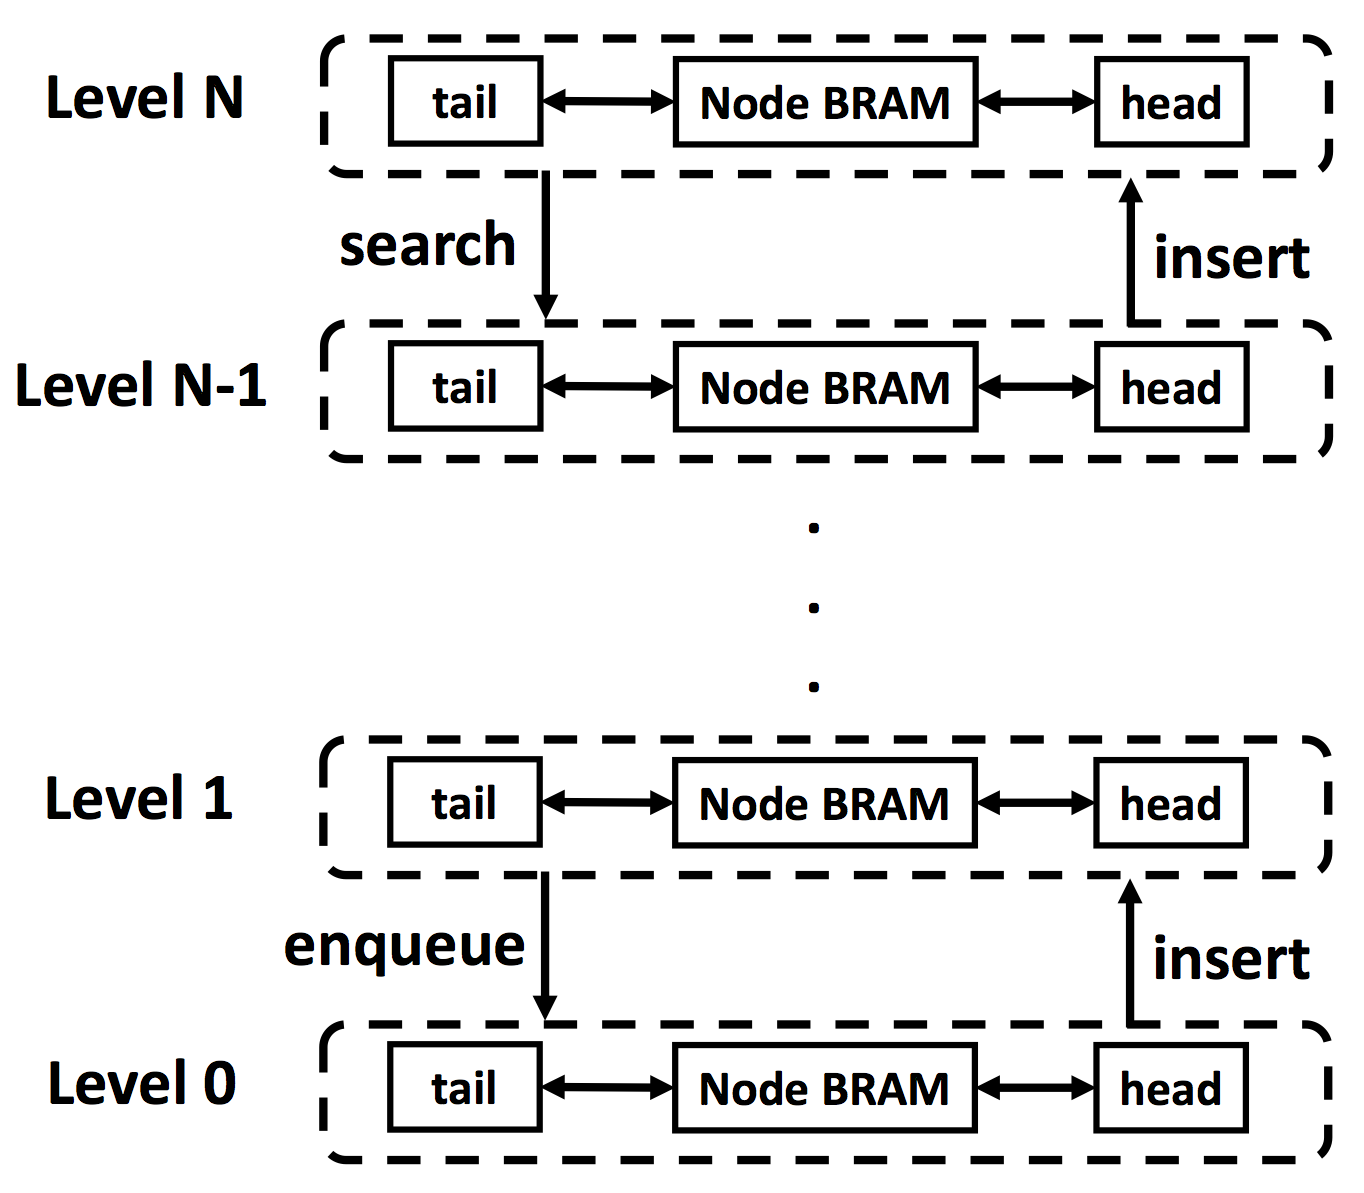
\includegraphics[width=0.8\linewidth]{figures/design/pipe-skip-list}
\caption{Pipelined skip list block diagram.}
\label{fig:pipe-skip-list}
\end{figure}


\subsection{Considerations for Future Scheduler Designs}
In order to make a real production scheduler programmable, one must take into consideration a number of additional features that we have not yet discussed in this paper.

\subsubsection*{Programmability of the Rank Computation}
During the evaluations presented in Section \ref{sec:sched-evals}, we assumed that the rank of each packet was correctly precomputed before arriving at the scheduler. A truly programmable scheduler must allow a developer to express that rank computation in a high-level way; for example, by writing a P4 program. Exactly how the rank computation should interact with the scheduler is non-obvious because it should take place after deciding whether or not to drop the packet. We believe that the P4 language will need to be extended to support a new type of architectural element that will facilitate the implementation of scheduling algorithms.

\subsubsection*{Hierarchical Scheduling Algorithms}
This paper only considers implementing algorithms for which the scheduling order of buffered packets does not change with arrival of future packets. This is consistent with the limitations on the sorts of algorithms that can be implemented using a single PIFO. However, as explained in \cite{pifo2016}, multiple PIFOs can be combined in a tree structure to facilitate the implementation of hierarchical scheduling algorithms, which can in fact cause reordering of packets that are already buffered. When combined into a tree, those PIFOs at the leaf positions store packet descriptors and all other PIFOs store pointers to one of their PIFO children. To enqueue a packet into a PIFO tree, it is first enqueued into the leaf PIFO and then a pointer to the current PIFO is enqueued into the parent all the way up to the root. A dequeue operation proceeds in exactly the opposite direction. Our PIFO design can be wired together into a tree structure, although additional consideration is needed to ensure that the full design will still be able to achieve line rate performance. A naive implementation would simply pipeline the various PIFO enqueue and dequeue operations, although this then requires multiple levels of bypass to ensure that recently enqueued packets can be immediately dequeued if necessary.

\subsubsection*{Non-Work-Conserving Scheduling Algorithms}
The authors of \cite{pifo2016} also discuss the idea of using an additional "shaping" PIFO to implement scheduling algorithms that require input rate limiting. These scheduling algorithms are non-work-conserving and specify the time at which packets should be enqueued, so they require an additional computation to determine this time, what the authors call a "shaping transaction". Presuming that this shaping transaction exists, we believe that our design can be easily extended with a mechanism that examines the current wall clock time before removing an element from the PIFO. This would help to facilitate the implementation of these non-work-conserving algorithms.


\subsubsection*{Alternate Drop Policies}
The design proposed in this paper implements the simplest, and most common, drop policy - tail drop. When using this policy, if an arriving packet encounters a full queue, it is dropped. There are also many other active queue management policies such as RED~\cite{red}, WRED~\cite{wred}, and REM~\cite{rem}. In particular, the one that we believe is most fitting for a PIFO implementation is to enqueue all arriving packets and then drop the one with the lowest priority (highest rank) if the queue exceeds a certain threshold. Dropping packets that are already in the buffer can be challenging, but we believe that it is feasible by extending our design to track the pointer to the head segment of packet with the lowest rank in each queue so that it can be removed if the queue reaches saturation.

\subsubsection*{Broadcasting and Multicasting}
A production scheduler implementation must be capable of supporting broadcasting and multicasting.  These can be implemented by modifying the packet buffer to support replication of packets to all or a subset of the output ports.

% \todo[inline]{Targeting an ASIC}






%%%%%%%%%%%%%%%%%%%%%%

%%%%%%%%%%%%%%%%%%%%%%
%%%%%%%%%%%%%%%%%%%%%%
\section{Related Work}
%%%%%%%%%%%%%%%%%%%%%%

Sivaraman et al.~\cite{pifo2016} present the PIFO as a useful abstraction for implementing many different scheduling algorithms. The authors also propose a hardware design for a PIFO targeting a 16-nm standard cell library. The proposed PIFO design uses per-flow FIFO queues stored in SRAM as well as a flip-flop based flow scheduler to sort the head packets of each flow. This design scales to support only about 1000 flows for an ASIC, and for an FPGA it would only be able to support about 64 flows. The reason is because the flow scheduler has very tight timing requirements which are difficult to meet on an FPGA. Additionally, the authors' proposed design makes the assumption that the rank values are monotonically increasing within a flow, which limits the granularity at which packets can be scheduled. It is for these reasons that we decided it was best to propose a completely new PIFO design for FPGAs. The PIFO design described in this paper makes no assumptions about the order of rank values within a flow and it can support as many flows as there are packet descriptors in the PIFO.

There is prior work that studies designs for line rate schedulers~\cite{pipelined-heap-2007,pheap-2000}. However, these studies have typically targeted ASIC devices, and assume that the scheduler uses per flow queuing. Additionally, they generally make use of heavy pipelining. As mentioned in section \ref{sec:optimizations}, pipelining is a design approach that is orthogonal to most of the techniques described in this paper.

There are few published prior works targeting FPGA, with two notable exceptions.  O'Neill et al.~\cite{belfast2011} presented a scalable modular traffic manager architecture, which was inspirational for our work, but pre-dated more modern notions of network programmability, and also targeted an FPGA of several generations ago, hence limiting the possible implementation results.  Benacer et al.~\cite{montreal2017} presented a fixed traffic manager architecture, with customization made possible through the use of high-level synthesis for a present-day FPGA.  However, this limited the possible clock rate to below 100MHz, with consequent adverse effect on line rate. 


 




%%%%%%%%%%%%%%%%%%%%%%

%%%%%%%%%%%%%%%%%%%%%%
%%%%%%%%%%%%%%%%%%%%%%
\section{Reproducibility}
%%%%%%%%%%%%%%%%%%%%%%

Along with the final version of the paper, we will make all of the hardware code available in an open source repository. We will also put together a virtual machine image with all of the necessary dependencies installed to make it easy for others to reproduce all of our simulation results.
%%%%%%%%%%%%%%%%%%%%%%
%%%%%%%%%%%%%%%%%%%%%%
\section{Conclusion}
%%%%%%%%%%%%%%%%%%%%%%

We are in the midst of a programmable networking revolution and we believe that tackling the challenge of programmable scheduling is a key next step. FPGAs greatly facilitate this design space exploration and have been one of the key platforms used to push the boundaries of programmable networking. The scheduler has very tight timing requirements, which makes them difficult to design and build. This is the main reason why modern packet processing devices offer a small menu of fixed scheduling algorithms that can only be slightly tuned and configured. By making the scheduling decision at the time of enqueue, the PIFO abstraction leads to both an efficient implementation and a mechanism with which to program many different scheduling algorithms. As we have demonstrated, a PIFO can be efficiently implemented on an FPGA which, we believe, will pave the way to further development of programmable scheduling.

%The scheduler has very tight timing requirements, which makes them difficult to design and build. This is the main reason why modern packet processing devices offer a small menu of fixed scheduling algorithms that can only be slightly tuned and configured. The PIFO queue implemented in FPGAs paves the way to further development of programmable scheduling using extensions to P4.





% \section{Introduction}

The \textit{proceedings} are the records of a conference.\footnote{This
  is a footnote}  ACM seeks
to give these conference by-products a uniform, high-quality
appearance.  To do this, ACM has some rigid requirements for the
format of the proceedings documents: there is a specified format
(balanced double columns), a specified set of fonts (Arial or
Helvetica and Times Roman) in certain specified sizes, a specified
live area, centered on the page, specified size of margins, specified
column width and gutter size.

\section{The Body of The Paper}
Typically, the body of a paper is organized into a hierarchical
structure, with numbered or unnumbered headings for sections,
subsections, sub-subsections, and even smaller sections.  The command
\texttt{{\char'134}section} that precedes this paragraph is part of
such a hierarchy.\footnote{This is a footnote.} \LaTeX\ handles the
numbering and placement of these headings for you, when you use the
appropriate heading commands around the titles of the headings.  If
you want a sub-subsection or smaller part to be unnumbered in your
output, simply append an asterisk to the command name.  Examples of
both numbered and unnumbered headings will appear throughout the
balance of this sample document.

Because the entire article is contained in the \textbf{document}
environment, you can indicate the start of a new paragraph with a
blank line in your input file; that is why this sentence forms a
separate paragraph.

\subsection{Type Changes and {\itshape Special} Characters}

We have already seen several typeface changes in this sample.  You can
indicate italicized words or phrases in your text with the command
\texttt{{\char'134}textit}; emboldening with the command
\texttt{{\char'134}textbf} and typewriter-style (for instance, for
computer code) with \texttt{{\char'134}texttt}.  But remember, you do
not have to indicate typestyle changes when such changes are part of
the \textit{structural} elements of your article; for instance, the
heading of this subsection will be in a sans serif\footnote{Another
  footnote here.  Let's make this a rather long one to see how it
  looks.} typeface, but that is handled by the document class file.
Take care with the use of\footnote{Another footnote.}  the
curly braces in typeface changes; they mark the beginning and end of
the text that is to be in the different typeface.

You can use whatever symbols, accented characters, or non-English
characters you need anywhere in your document; you can find a complete
list of what is available in the \textit{\LaTeX\ User's Guide}
\cite{Lamport:LaTeX}.

\subsection{Math Equations}
You may want to display math equations in three distinct styles:
inline, numbered or non-numbered display.  Each of
the three are discussed in the next sections.

\subsubsection{Inline (In-text) Equations}
A formula that appears in the running text is called an
inline or in-text formula.  It is produced by the
\textbf{math} environment, which can be
invoked with the usual \texttt{{\char'134}begin\,\ldots{\char'134}end}
construction or with the short form \texttt{\$\,\ldots\$}. You
can use any of the symbols and structures,
from $\alpha$ to $\omega$, available in
\LaTeX~\cite{Lamport:LaTeX}; this section will simply show a
few examples of in-text equations in context. Notice how
this equation:
\begin{math}
  \lim_{n\rightarrow \infty}x=0
\end{math},
set here in in-line math style, looks slightly different when
set in display style.  (See next section).

\subsubsection{Display Equations}
A numbered display equation---one set off by vertical space from the
text and centered horizontally---is produced by the \textbf{equation}
environment. An unnumbered display equation is produced by the
\textbf{displaymath} environment.

Again, in either environment, you can use any of the symbols
and structures available in \LaTeX\@; this section will just
give a couple of examples of display equations in context.
First, consider the equation, shown as an inline equation above:
\begin{equation}
  \lim_{n\rightarrow \infty}x=0
\end{equation}
Notice how it is formatted somewhat differently in
the \textbf{displaymath}
environment.  Now, we'll enter an unnumbered equation:
\begin{displaymath}
  \sum_{i=0}^{\infty} x + 1
\end{displaymath}
and follow it with another numbered equation:
\begin{equation}
  \sum_{i=0}^{\infty}x_i=\int_{0}^{\pi+2} f
\end{equation}
just to demonstrate \LaTeX's able handling of numbering.

\subsection{Citations}
Citations to articles~\cite{bowman:reasoning,
clark:pct, braams:babel, herlihy:methodology},
conference proceedings~\cite{clark:pct} or maybe
books \cite{Lamport:LaTeX, salas:calculus} listed
in the Bibliography section of your
article will occur throughout the text of your article.
You should use BibTeX to automatically produce this bibliography;
you simply need to insert one of several citation commands with
a key of the item cited in the proper location in
the \texttt{.tex} file~\cite{Lamport:LaTeX}.
The key is a short reference you invent to uniquely
identify each work; in this sample document, the key is
the first author's surname and a
word from the title.  This identifying key is included
with each item in the \texttt{.bib} file for your article.

The details of the construction of the \texttt{.bib} file
are beyond the scope of this sample document, but more
information can be found in the \textit{Author's Guide},
and exhaustive details in the \textit{\LaTeX\ User's
Guide} by Lamport~\shortcite{Lamport:LaTeX}.

This article shows only the plainest form
of the citation command, using \texttt{{\char'134}cite}.

Some examples.  A paginated journal article \cite{Abril07}, an enumerated
journal article \cite{Cohen07}, a reference to an entire issue \cite{JCohen96},
a monograph (whole book) \cite{Kosiur01}, a monograph/whole book in a series (see 2a in spec. document)
\cite{Harel79}, a divisible-book such as an anthology or compilation \cite{Editor00}
followed by the same example, however we only output the series if the volume number is given
\cite{Editor00a} (so Editor00a's series should NOT be present since it has no vol. no.),
a chapter in a divisible book \cite{Spector90}, a chapter in a divisible book
in a series \cite{Douglass98}, a multi-volume work as book \cite{Knuth97},
an article in a proceedings (of a conference, symposium, workshop for example)
(paginated proceedings article) \cite{Andler79}, a proceedings article
with all possible elements \cite{Smith10}, an example of an enumerated
proceedings article \cite{VanGundy07},
an informally published work \cite{Harel78}, a doctoral dissertation \cite{Clarkson85},
a master's thesis: \cite{anisi03}, an online document / world wide web
resource \cite{Thornburg01, Ablamowicz07, Poker06}, a video game (Case 1) \cite{Obama08} and (Case 2) \cite{Novak03}
and \cite{Lee05} and (Case 3) a patent \cite{JoeScientist001},
work accepted for publication \cite{rous08}, 'YYYYb'-test for prolific author
\cite{SaeediMEJ10} and \cite{SaeediJETC10}. Other cites might contain
'duplicate' DOI and URLs (some SIAM articles) \cite{Kirschmer:2010:AEI:1958016.1958018}.
Boris / Barbara Beeton: multi-volume works as books
\cite{MR781536} and \cite{MR781537}.

A couple of citations with DOIs: \cite{2004:ITE:1009386.1010128,
  Kirschmer:2010:AEI:1958016.1958018}.

Online citations: \cite{TUGInstmem, Thornburg01, CTANacmart}.


\subsection{Tables}
Because tables cannot be split across pages, the best
placement for them is typically the top of the page
nearest their initial cite.  To
ensure this proper ``floating'' placement of tables, use the
environment \textbf{table} to enclose the table's contents and
the table caption.  The contents of the table itself must go
in the \textbf{tabular} environment, to
be aligned properly in rows and columns, with the desired
horizontal and vertical rules.  Again, detailed instructions
on \textbf{tabular} material
are found in the \textit{\LaTeX\ User's Guide}.

Immediately following this sentence is the point at which
Table~\ref{tab:freq} is included in the input file; compare the
placement of the table here with the table in the printed
output of this document.

\begin{table}
  \caption{Frequency of Special Characters}
  \label{tab:freq}
  \begin{tabular}{ccl}
    \toprule
    Non-English or Math&Frequency&Comments\\
    \midrule
    \O & 1 in 1,000& For Swedish names\\
    $\pi$ & 1 in 5& Common in math\\
    \$ & 4 in 5 & Used in business\\
    $\Psi^2_1$ & 1 in 40,000& Unexplained usage\\
  \bottomrule
\end{tabular}
\end{table}

To set a wider table, which takes up the whole width of the page's
live area, use the environment \textbf{table*} to enclose the table's
contents and the table caption.  As with a single-column table, this
wide table will ``float'' to a location deemed more desirable.
Immediately following this sentence is the point at which
Table~\ref{tab:commands} is included in the input file; again, it is
instructive to compare the placement of the table here with the table
in the printed output of this document.


\begin{table*}
  \caption{Some Typical Commands}
  \label{tab:commands}
  \begin{tabular}{ccl}
    \toprule
    Command &A Number & Comments\\
    \midrule
    \texttt{{\char'134}author} & 100& Author \\
    \texttt{{\char'134}table}& 300 & For tables\\
    \texttt{{\char'134}table*}& 400& For wider tables\\
    \bottomrule
  \end{tabular}
\end{table*}
% end the environment with {table*}, NOTE not {table}!

It is strongly recommended to use the package booktabs~\cite{Fear05}
and follow its main principles of typography with respect to tables:
\begin{enumerate}
\item Never, ever use vertical rules.
\item Never use double rules.
\end{enumerate}
It is also a good idea not to overuse horizontal rules.


\subsection{Figures}

Like tables, figures cannot be split across pages; the best placement
for them is typically the top or the bottom of the page nearest their
initial cite.  To ensure this proper ``floating'' placement of
figures, use the environment \textbf{figure} to enclose the figure and
its caption.

This sample document contains examples of \texttt{.eps} files to be
displayable with \LaTeX.  If you work with pdf\LaTeX, use files in the
\texttt{.pdf} format.  Note that most modern \TeX\ systems will convert
\texttt{.eps} to \texttt{.pdf} for you on the fly.  More details on
each of these are found in the \textit{Author's Guide}.

\begin{figure}
\includegraphics{fly}
\caption{A sample black and white graphic.}
\end{figure}

\begin{figure}
\includegraphics[height=1in, width=1in]{fly}
\caption{A sample black and white graphic
that has been resized with the \texttt{includegraphics} command.}
\end{figure}


As was the case with tables, you may want a figure that spans two
columns.  To do this, and still to ensure proper ``floating''
placement of tables, use the environment \textbf{figure*} to enclose
the figure and its caption.  And don't forget to end the environment
with \textbf{figure*}, not \textbf{figure}!

\begin{figure*}
\includegraphics{flies}
\caption{A sample black and white graphic
that needs to span two columns of text.}
\end{figure*}


\begin{figure}
\includegraphics[height=1in, width=1in]{rosette}
\caption{A sample black and white graphic that has
been resized with the \texttt{includegraphics} command.}
\end{figure}

\subsection{Theorem-like Constructs}

Other common constructs that may occur in your article are the forms
for logical constructs like theorems, axioms, corollaries and proofs.
ACM uses two types of these constructs:  theorem-like and
definition-like.

Here is a theorem:
\begin{theorem}
  Let $f$ be continuous on $[a,b]$.  If $G$ is
  an antiderivative for $f$ on $[a,b]$, then
  \begin{displaymath}
    \int^b_af(t)\,dt = G(b) - G(a).
  \end{displaymath}
\end{theorem}

Here is a definition:
\begin{definition}
  If $z$ is irrational, then by $e^z$ we mean the
  unique number that has
  logarithm $z$:
  \begin{displaymath}
    \log e^z = z.
  \end{displaymath}
\end{definition}

The pre-defined theorem-like constructs are \textbf{theorem},
\textbf{conjecture}, \textbf{proposition}, \textbf{lemma} and
\textbf{corollary}.  The pre-defined de\-fi\-ni\-ti\-on-like constructs are
\textbf{example} and \textbf{definition}.  You can add your own
constructs using the \textsl{amsthm} interface~\cite{Amsthm15}.  The
styles used in the \verb|\theoremstyle| command are \textbf{acmplain}
and \textbf{acmdefinition}.

Another construct is \textbf{proof}, for example,

\begin{proof}
  Suppose on the contrary there exists a real number $L$ such that
  \begin{displaymath}
    \lim_{x\rightarrow\infty} \frac{f(x)}{g(x)} = L.
  \end{displaymath}
  Then
  \begin{displaymath}
    l=\lim_{x\rightarrow c} f(x)
    = \lim_{x\rightarrow c}
    \left[ g{x} \cdot \frac{f(x)}{g(x)} \right ]
    = \lim_{x\rightarrow c} g(x) \cdot \lim_{x\rightarrow c}
    \frac{f(x)}{g(x)} = 0\cdot L = 0,
  \end{displaymath}
  which contradicts our assumption that $l\neq 0$.
\end{proof}

\section{Conclusions}
This paragraph will end the body of this sample document.
Remember that you might still have Acknowledgments or
Appendices; brief samples of these
follow.  There is still the Bibliography to deal with; and
we will make a disclaimer about that here: with the exception
of the reference to the \LaTeX\ book, the citations in
this paper are to articles which have nothing to
do with the present subject and are used as
examples only.
%\end{document}  % This is where a 'short' article might terminate



\appendix
%Appendix A
\section{Headings in Appendices}
The rules about hierarchical headings discussed above for
the body of the article are different in the appendices.
In the \textbf{appendix} environment, the command
\textbf{section} is used to
indicate the start of each Appendix, with alphabetic order
designation (i.e., the first is A, the second B, etc.) and
a title (if you include one).  So, if you need
hierarchical structure
\textit{within} an Appendix, start with \textbf{subsection} as the
highest level. Here is an outline of the body of this
document in Appendix-appropriate form:
\subsection{Introduction}
\subsection{The Body of the Paper}
\subsubsection{Type Changes and  Special Characters}
\subsubsection{Math Equations}
\paragraph{Inline (In-text) Equations}
\paragraph{Display Equations}
\subsubsection{Citations}
\subsubsection{Tables}
\subsubsection{Figures}
\subsubsection{Theorem-like Constructs}
\subsubsection*{A Caveat for the \TeX\ Expert}
\subsection{Conclusions}
\subsection{References}
Generated by bibtex from your \texttt{.bib} file.  Run latex,
then bibtex, then latex twice (to resolve references)
to create the \texttt{.bbl} file.  Insert that \texttt{.bbl}
file into the \texttt{.tex} source file and comment out
the command \texttt{{\char'134}thebibliography}.
% This next section command marks the start of
% Appendix B, and does not continue the present hierarchy
\section{More Help for the Hardy}

Of course, reading the source code is always useful.  The file
\path{acmart.pdf} contains both the user guide and the commented
code.

\begin{acks}
  The authors would like to thank Dr. Yuhua Li for providing the
  MATLAB code of the \textit{BEPS} method.

  The authors would also like to thank the anonymous referees for
  their valuable comments and helpful suggestions. The work is
  supported by the \grantsponsor{GS501100001809}{National Natural
    Science Foundation of
    China}{http://dx.doi.org/10.13039/501100001809} under Grant
  No.:~\grantnum{GS501100001809}{61273304}
  and~\grantnum[http://www.nnsf.cn/youngscientists]{GS501100001809}{Young
    Scientists' Support Program}.

\end{acks}


\bibliographystyle{ACM-Reference-Format}
\bibliography{references}
%\bibliography{sample-bibliography}

\end{document}
